% !TeX root = index.tex

\documentclass{scrreprt}

\newcommand{\varVersion}{0.1}

\newcommand{\varAuthor}{Oliver Thoma}
\newcommand{\varTitle}{Renuo Assessment-Assistant}
\newcommand{\varSubtitle}{IPA-Bericht vom 23.05.2022 bis 07.06.2022}
\newcommand{\varCompany}{Renuo AG} 
\newcommand{\varCompanyDepartment}{wg-interns}

\newcommand{\varCandidate}{
  \textbf{\varAuthor} \\ oliver.thoma@renuo.ch \\ 076 362 50 05 (P) \\ 044 500 83 50 (G)
}
\newcommand{\varResponsibleSpecialist}{
  \textbf{Simon Huber} \\ simon.huber@renuo.ch \\ 044 500 83 53 (G)
}
\newcommand{\varVocationalTrainer}{
  \textbf{Rima Kalberer} \\ rima.kalberer@kbw.ch \\  076 595 95 38 (P) 
}
\newcommand{\varPrimaryExpert}{
  \textbf{Christian Mäder} \\ pk19@cmaeder.ch \\ 079 524 51 83 (P) 
}
\newcommand{\varSecondaryExpert}{
  \textbf{Roberto Ranieri} \\ roberto.ranieri@gmx.net \\  079 349 30 74 (P) 
}
\newcommand{\varExaminationBoard}{Prüfungskomission 19} % Prüfungsorganisation
\newcommand{\varExaminationBoardDepartment}{Informatik Applikationsentwicklung} % Fachrichtung

% apply ipa package
\usepackage{../lib/ipa}

\lohead[\varTitle]{\varTitle}
\lofoot[\today]{\today}
% see B6.5
\cfoot[\varAuthor\ / \varCompany\\Version \varVersion ]{\varAuthor\ / \varCompany\\Version \varVersion}
\rofoot[Seite \pagemark{} von \pageref{LastPage}]{Seite \pagemark{} von \pageref{LastPage}}

% load sources
\addbibresource{sources.bib}

% make glossaries
\makenoidxglossaries

% define glossary entries
% see B6.6
\newglossaryentry{Organigramm}
{
  name={Organigramm},
  description={Ein Organigramm stellt eine Organisation und deren Aufbauorganisation grafisch dar.}
}

\newglossaryentry{cicd}
{
  name={CI/CD},
  description={Bei der \emph{Continuous Integration} (CI) wird der Source Code mit dem restlichen Source Code zusammengeführt, gebaut und getestet.
      Beim \emph{Continuous Deployment} (CD) wird das Software Paket automatisch in die Produktion deployed.}
}


% create document
\begin{document}

% set page numbering
\pagenumbering{roman}

% set page style
\pagestyle{scrheadings}

% include title page
\thispagestyle{empty}

\begin{center}
  \makebox[\textwidth]{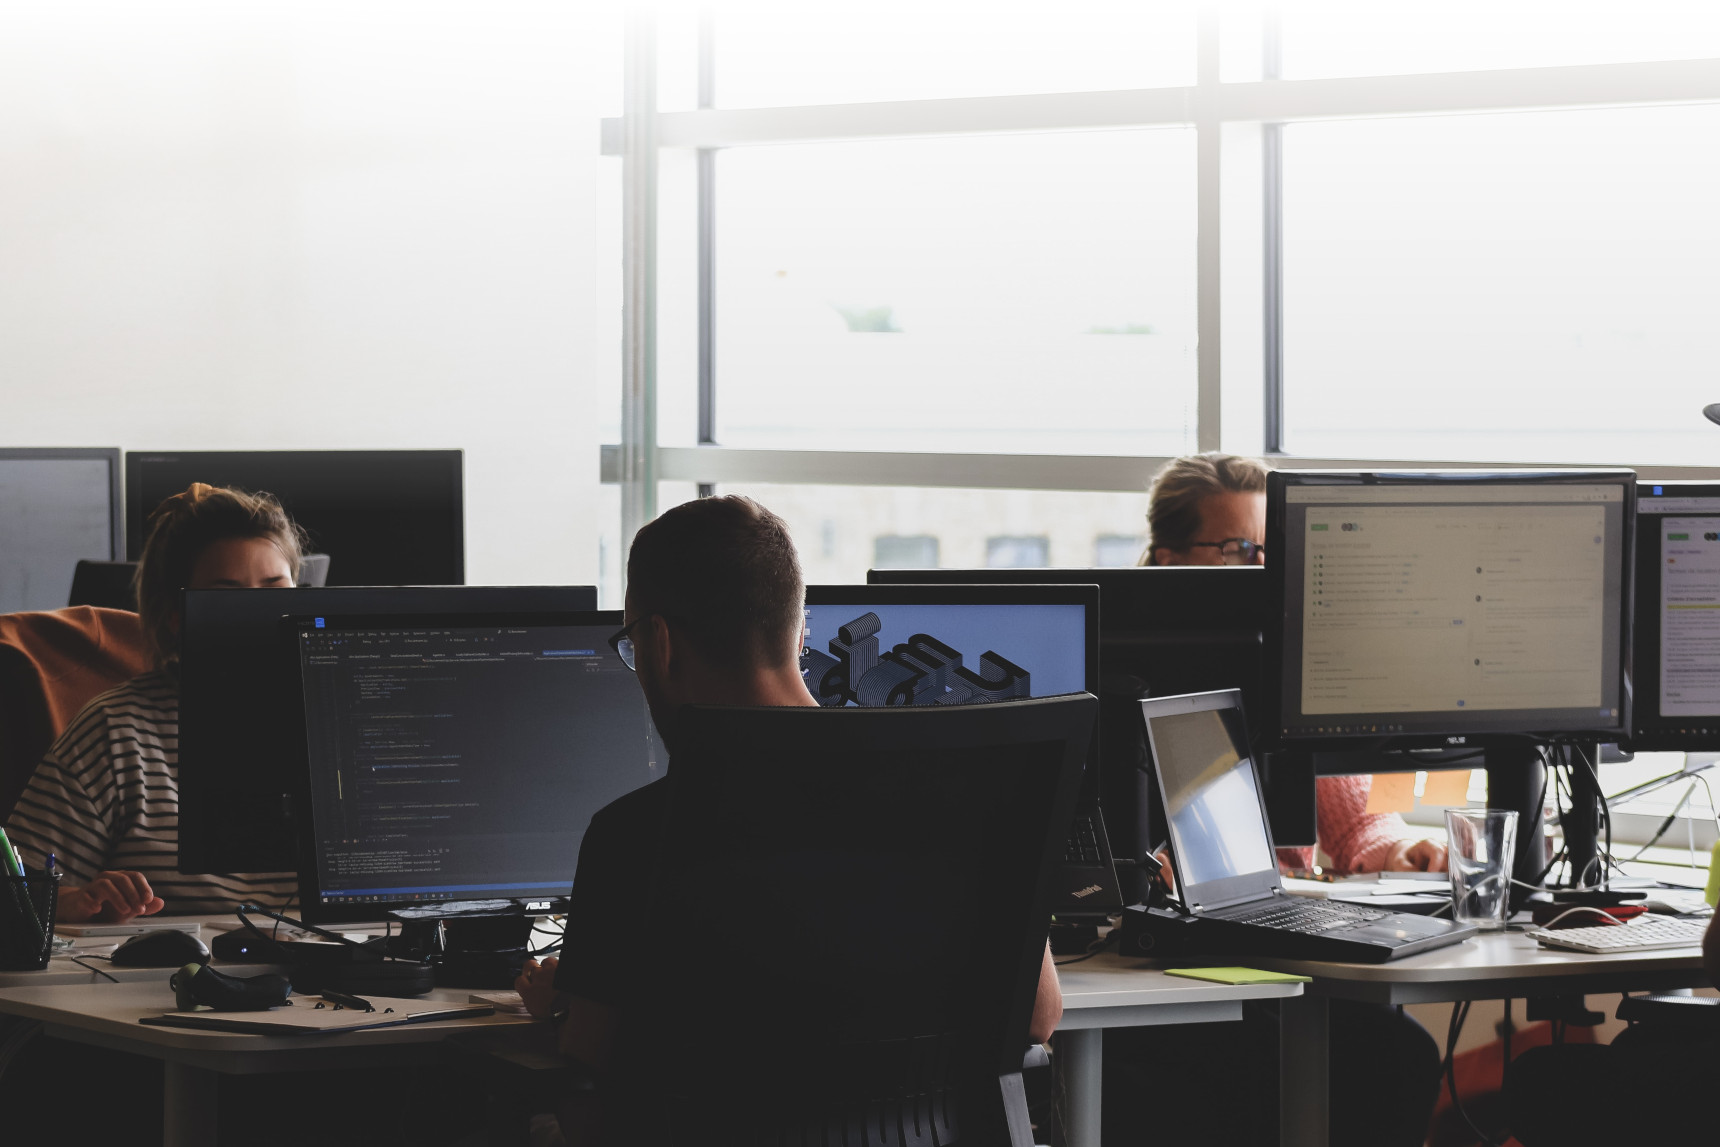
\includegraphics[width=1.1\paperwidth]{images/title.jpg}}
\end{center}
\vspace*{1cm}
{\fontsize{28}{28}\selectfont \varTitle}\\[0.25cm]
{\fontsize{16}{16}\selectfont \varAuthor}\\[0.25cm]
{\fontsize{16}{16}\selectfont \varCompany}

\newpage
\TileWallPaper{\paperwidth}{\paperheight}{images/background.pdf}

% see A1.3
% see B6.3
% generate the table of contents
\tableofcontents

% finish page
\clearpage

% use the arabic numbering system
\pagenumbering{arabic}

% reset page counter
\setcounter{page}{1}

% see B6.1a
% create a phantom toc entry for "Umfeld und Ablauf"
\clearpage\phantomsection\addcontentsline{toc}{part}{Umfeld und Ablauf (Teil 1)}

% [2]: Seite 11
\chapter{Aufgabenstellung}

Dieses Kapitel beinhaltet die komplette Aufgabenstellung im originalen Wortlaut von PkOrg.ch.

\section{Ausgangslage}

Der Einstellungsprozess der Renuo ist zeitaufwendig wegen der intensiven Assessments, welche Bewerber
durchlaufen müssen. So unterziehen sich z.B. IMS-Praktikanten (8 Assessments bei etwa 40 Bewerbern) einer
vierstündigen Session mit 12 Programmieraufgaben. Diese Aufgaben werden gewissenhaft korrigiert. Die
Resultate werden den Bewerbern mitgeteilt, sodass die investierte Zeit bei jedem Ausgang des Assessments
nicht vergebens ist.

Diese IPA hat zum Ziel die Koordination des Renuo-Assessment-Prozesses mit einer Web-Plattform zu
erleichtern. Das Austeilen der Aufgaben und die rechtzeitige Abgabe der Lösungen soll vereinheitlicht werden.
Im Weiteren sollen die Aufgaben neu direkt in der Plattform erfasst und die Lösungen ausgewertet werden
können.

\section{Detaillierte Aufgabenstellung}

Die in dieser Arbeit entwickelte Web-Plattform vereinheitlicht und erleichtert den Renuo-Assessment-Prozess.

\textbf{Die Software bedient folgende Benutzerrollen:}
\begin{itemize}
    \item \enquote{Bewerber}: durchläuft ein Assessment
    \item \enquote{Betreuer}: koordiniert den Ablauf des Assessments
    \item \enquote{Korrektor}: korrigiert die Lösungen
\end{itemize}

\emph{(Die Rollen des Betreuers und des Korrektors müssen nicht separat gehandhabt werden.)}

\newpage

\subsection{Funktionale Anforderungen}

\begin{itemize}
    \item F1: \enquote{Als Bewerber kann ich per Einladungs-Link an einer Assessment-Session teilnehmen} (damit ich Zugriff auf die Aufgaben erhalte.)
    \item F2: \enquote{Als Bewerber sehe ich, wie lange die Assessment-Session dauert, damit ich mir meine Arbeit richtig aufteilen kann.}
    \item F3: \enquote{Als Bewerber kann ich meine Lösungen zu jeder Aufgabe einzeln hochladen damit meine Leistung mit den der anderen Bewerber verglichen werden kann.}
          \\Die Aufgaben können wie folgt abgegeben werden:
          \begin{itemize}
              \item als Dateien (z.B. Fotos von handgezeichneten Diagrammen)
          \end{itemize}
    \item F4: \enquote{Als Bewerber erhalte ich nach dem Assessment Einsicht in den Korrektur-Kommentar.}
    \item F5: \enquote{Als Betreuer kann ich Assessment-Sessionen konfigurieren. So kontrolliere ich wann und wie lange das Assessment stattfindet und wer daran teilnimmt.}
          \begin{itemize}
              \item Bewerber werden per E-Mail-Adresse erfasst.
              \item Die Assessment-Session durchläuft folgende Status: \emph{preparing, open, reviewing, closed}
              \item Es können beliebig viele Assessment-Sessionen laufen - auch gleichzeitig.
          \end{itemize}
    \item F6: \enquote{Als Betreuer kann ich zu einer Assessment-Sessionen Aufgaben mit einer Beschreibung verwalten.}
          \begin{itemize}
              \item Die Beschreibung kann formatiert werden (HTML / Markdown)
              \item Als Bewerber kann ich die Aufgabenstellung im Portal einsehen
          \end{itemize}
    \item F7: \enquote{Als Betreuer kann ich Bewerber per Instruktions-E-Mail mit Invite-Link zu einer Assessment-Session einladen. So stelle ich sicher, dass die Bewerber rechtzeitig informiert sind und sich auf die Session vorbereiten können.}
          \begin{itemize}
              \item Die E-Mail soll die E-Mail-Adresse des Betreuers im reply-to-Header enthalten.
              \item Der E-Mail-Inhalt darf hardcoded sein
          \end{itemize}
    \item F8: \enquote{Als Korrektor kann ich pro Assessment-Session jede Aufgabe mit den dazu abgegebenen Lösungen einsehen und Korrektur-Kommentare abgeben.}
          \begin{itemize}
              \item Die Korrektur findet pro Aufgabe und nicht pro Person statt, damit ein Vergleich zwischen den Kandidaten möglich ist
              \item Die Reihenfolge der Lösungen ist bei jeder Aufgabe zufällig
          \end{itemize}
    \item F9: \enquote{Als Korrektor sehe ich während der Korrektur nie, zu wem (E-Mail-Adresse) die abgegebene Lösung gehört. So bleibe ich unparteiisch.}
    \item F10: \enquote{Als Korrektor kann ich die Assessment-Session schliessen um den Bewerbungsprozess zu einer Entscheidung zu bringen.}
          \begin{itemize}
              \item Das generiert eine Tabelle mit allen Korrektur-Kommentaren pro Person.
              \item Der Bewerber kann seine Resultate auf dem Portal einsehen
          \end{itemize}
\end{itemize}

\newpage

\subsection{Nicht-funktionale Anforderungen}

\begin{itemize}
    \item N1 Software-Design: Die Applikation ist für Heroku (12factor) mit AWS S3-Speicher konzipiert.
    \item N2 Software-Design: Die Applikation ist versendet E-Mails via Sparkpost.
    \item N3 Sicherheit: Bewerber dürfen die Lösungen anderer Bewerber nicht sehen können. Die Öffentlichkeit hat niemals Zugriff auf Aufgaben oder Lösungen.
    \item N4 Performance: Das Hochladen von (auch grossen) Dateien darf den Betrieb für Bewerber nicht beeinträchtigen.
    \item N5 UX: Für die Bedienung darf kein dediziertes Benutzerhandbuch notwendig sein.
    \item N6 Dokumentation: Wichtige Teile der Software müssen mit den richtigen UML-Diagrammen beschrieben werden:
          \begin{itemize}
              \item Entity-Relation-Diagramm für die Business-Domain
              \item State-Diagramm (Zustandsdiagramm) zur Kontrolle des Assessment-Ablaufs
          \end{itemize}
    \item N7 Tests: Der Happy-Path für alle Rollen muss automatisiert getestet sein (UI-Tests).
    \item N8 Tests: Die Unit-Test-Abdeckung des geschriebenen Codes beträgt 100%.
\end{itemize}

\section{Mittel und Methoden}

\textbf{Für die IPA werden folgende Technologien eingesetzt:}
\begin{itemize}
    \item Ruby on Rails
    \item HTML5 (HTML, JS, CSS)
\end{itemize}

% [2]: Seite 11
\chapter{Deklaration}

Folgender Abschnitt beschreibt die Vorkenntnisse des Kandidaten und dessen Vorbereitung.

\section{Vorkenntnisse}

Der Lernende hat seit Praktikumsbeginn (2. August 2021) mit Ruby on Rails gearbeitet. Auch wurden die Tests in dieser Zeit mit RSpec und Capybara geschrieben und die Code-Qualität mit Rubocop überprüft.
Ebenfalls seit Praktikumsstart wurde Git und Git Flow zusammen mit Github eingesetzt. Code-Reviews gehören ebenfalls zur täglichen Arbeit (sowohl Code Reviews durchführen, wie auch entgegennehmen).
Heroku und SemaphoreCI werden ebenfalls seit Praktikumsbeginn eingesetzt.

\section{Vorarbeiten}

Zur Vorbereitung der IPA wird ein vollständiges App-Setup nach dem Renuo App-Setup-Guide gemacht.

\textbf{Dafür wird folgendes gemacht:}
\begin{itemize}
    \item Generieren einer vanilla Ruby on Rails Applikation mittels \mintinline{bash}{rails new}
    \item Einrichten von GitHub repository und allen Branches nach GitFlow
    \item Installieren von grundlegenden Abhängigkeiten. Dazu gehören z.B. die Testumgebung \emph{rspec},
          das CSS-Framework \emph{bootstrap} oder \emph{simple\_form} für ein vereinfachtes generieren von Formularen.
    \item Einrichten der CI/CD-Pipelines auf SemaphoreCI inkl. Deployment auf Heroku
    \item Den E-Mail Service Sparkpost einbinden
    \item Einen AWS S3 Storage Bucket einrichten, um die File-Uploads speichern zu können.
\end{itemize}

\section{Neue Lerninhalte}

Die Aufgabenstellung beinhaltet grundsätzlich keine neuen Lerninhalte. Allenfalls hat der Kandidat noch nie mit formatierten Text-Inhalten und verschiedenen States gearbeitet. Dies ist aber mithilfe von etwas Recherche gut lösbar.

\section{Arbeiten in den letzten 6 Monaten}

Im Herbst 2021 wurde hauptsächlich mit Ruby on Rails gearbeitet. Das grösste Projekt war eine Plattform (core-values) um die zentralen Werte einer Firma zu ermitteln.
Dazu wurde Rails und Stimulus verwendet. In den letzten Monaten wurde in einem Kundenprojekt mit Java (Spring) und Angular (Typescript) gearbeitet, daneben auch mit Ruby on Rails an unserem internen Projekt “Gifcoins”.

\section{Eingesetzte Tools}

Ein modernes MacBook Pro mit der neusten macOS Version wird sowohl für die Entwicklung als auch für die Dokumentation eingesetzt.

\subsection{Dokumentation und Projektmanagement}

\begin{itemize}
    \item Um die Arbeitszeiten des Kandidaten einzutragen, wird redmine mit dem Tracky Plugin verwendet.
    \item Der IPA-Bericht wird in LaTeX verfasst. Dazu verwendet der Kandidat Visual Studio Code mit diversen Erweiterungen.
          Der Bericht baut auf der Vorlage \cite{Buhler_ipa-template_2022} auf.
    \item Sowohl umletino als auch das textbasierte Tool mermaid werden für UML-Diagramme verwendet.
\end{itemize}

\subsection{Entwicklung}

\begin{itemize}
    \item Die (Haupt-) Entwicklungsumgebung, die zum Einsatz kommt, ist JetBrains RubyMine.
    \item Fork wird als grafischer Git-Client eingesetzt.
    \item iTerm \& Alacritty als Terminal
    \item Der Kandidat verwendet sowohl Firefox als auch einen Chromium-basierten Browser während der Entwicklung, um eine Kompatibilität über alle Browser sicherzustellen.
\end{itemize}

% see B6.2a
\chapter{Projektaufbauorganisation}

Im Unterschied zur üblichen Arbeit im Betrieb werden zwei Experten die Arbeit des Kandidaten Begleiten und Bewerten.
Die Projektaufbauorganisation ist in \ref{fig:organigram} visualisiert.

\vspace*{0.5cm}

\begin{figure}[H]
  \begin{multicols}{2}
    \begin{forest}
      for tree={draw,grow'=0,folder,align=left}
      [\textbf{\varCompany} \emph{(Durchführungsort)}
        [\textbf{\varCompanyDepartment}
          [(VF) \\ \varResponsibleSpecialist]
          [(K) \\ \varCandidate]
        ]
      ]
    \end{forest}

    \begin{forest}
      for tree={draw,grow'=0,folder,align=left}
      [\textbf{\varExaminationBoard}
        [\textbf{\varExaminationBoardDepartment}
          [(HEX) \\ \varPrimaryExpert]
          [(NEX) \\ \varSecondaryExpert]
        ]
      ]
    \end{forest}
  \end{multicols}
  \begin{center}
    \begin{forest}
      for tree={draw,grow'=0,folder,align=left}
      [\textbf{Kantonsschule Büelrain Winterthur}
        [\textbf{Informatikmittelschule (IMS)}
          [(BB) \\ \varVocationalTrainer]
        ]
      ]
    \end{forest}
  \end{center}
  \caption[\enquote{Organigramm der am Projekt teilnehmenden Personen} visualisiert mit TikZ Forest]{\gls{Organigramm} der am Projekt teilnehmenden Personen}
  \label{fig:organigram}
\end{figure}

% see A1.2
% see A3
% see B6.2b
\begin{landscape}
  \chapter{Zeitplan}
  Der Zeitplan basiert auf der Vorlage \cite{Buhler_ipa-timetable_2022} und zeigt mit einer Auflösung von zwei Stundenblöcken die geplanten und getätigten Aufwände.
  \begin{figure}[H]
    \begin{center}
      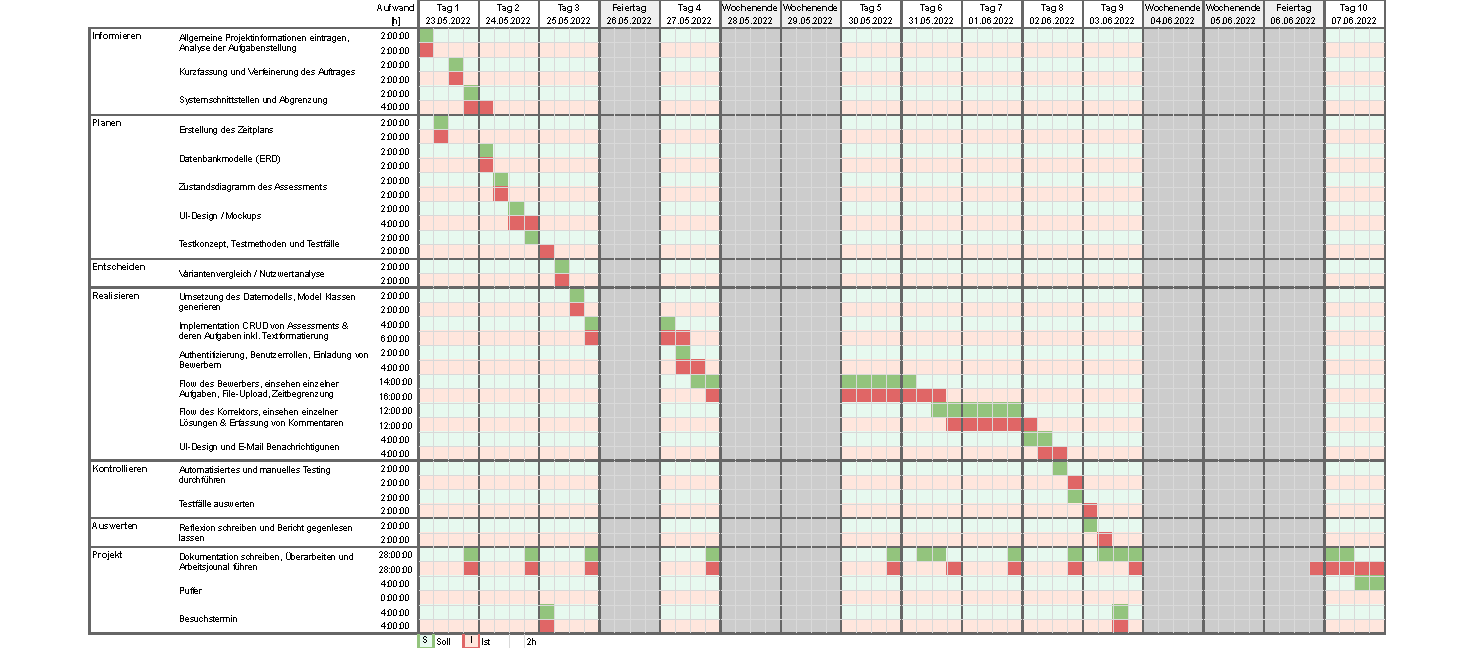
\includegraphics[width=1.55\textheight]{../res/timeplan.pdf}
    \end{center}
    \caption[\enquote{Zeitplan} erstellt mit Google Sheets]{Zeitplan}
    \label{fig:timeplan}
  \end{figure}
\end{landscape}

% see A2.1
% see B6.2c
\chapter{Arbeitsjournal}

\section{Tag 1}
\begin{tabularx}{\textwidth}[H]{|c|X|}
  \hline
  Erledigte Arbeiten & \lipsum[23] \\ \hline
  Ungeplante Arbeiten & \lipsum[24] \\ \hline
  Erfolge & \lipsum[25] \\ \hline
  Misserfolge & \lipsum[26] \\ \hline
  Hilfestellungen & \lipsum[27] \\
  \hline
\end{tabularx}

\newpage

\section{Tag 2}
\begin{tabularx}{\textwidth}[H]{|c|X|}
  \hline
  Erledigte Arbeiten & \lipsum[23] \\ \hline
  Ungeplante Arbeiten & \lipsum[24] \\ \hline
  Erfolge & \lipsum[25] \\ \hline
  Misserfolge & \lipsum[26] \\ \hline
  Hilfestellungen & \lipsum[27] \\
  \hline
\end{tabularx}

\newpage

\section{Tag 3}
\begin{tabularx}{\textwidth}[H]{|c|X|}
  \hline
  Erledigte Arbeiten & \lipsum[23] \\ \hline
  Ungeplante Arbeiten & \lipsum[24] \\ \hline
  Erfolge & \lipsum[25] \\ \hline
  Misserfolge & \lipsum[26] \\ \hline
  Hilfestellungen & \lipsum[27] \\
  \hline
\end{tabularx}

\newpage

\section{Tag 4}
\begin{tabularx}{\textwidth}[H]{|c|X|}
  \hline
  Erledigte Arbeiten & \lipsum[23] \\ \hline
  Ungeplante Arbeiten & \lipsum[24] \\ \hline
  Erfolge & \lipsum[25] \\ \hline
  Misserfolge & \lipsum[26] \\ \hline
  Hilfestellungen & \lipsum[27] \\
  \hline
\end{tabularx}

\newpage

\section{Tag 5}
\begin{tabularx}{\textwidth}[H]{|c|X|}
  \hline
  Erledigte Arbeiten & \lipsum[23] \\ \hline
  Ungeplante Arbeiten & \lipsum[24] \\ \hline
  Erfolge & \lipsum[25] \\ \hline
  Misserfolge & \lipsum[26] \\ \hline
  Hilfestellungen & \lipsum[27] \\
  \hline
\end{tabularx}

\newpage

\section{Tag 6}
\begin{tabularx}{\textwidth}[H]{|c|X|}
  \hline
  Erledigte Arbeiten & \lipsum[23] \\ \hline
  Ungeplante Arbeiten & \lipsum[24] \\ \hline
  Erfolge & \lipsum[25] \\ \hline
  Misserfolge & \lipsum[26] \\ \hline
  Hilfestellungen & \lipsum[27] \\
  \hline
\end{tabularx}

\newpage

\section{Tag 7}
\begin{tabularx}{\textwidth}[H]{|c|X|}
  \hline
  Erledigte Arbeiten & \lipsum[23] \\ \hline
  Ungeplante Arbeiten & \lipsum[24] \\ \hline
  Erfolge & \lipsum[25] \\ \hline
  Misserfolge & \lipsum[26] \\ \hline
  Hilfestellungen & \lipsum[27] \\
  \hline
\end{tabularx}

\newpage

\section{Tag 8}
\begin{tabularx}{\textwidth}[H]{|c|X|}
  \hline
  Erledigte Arbeiten & \lipsum[23] \\ \hline
  Ungeplante Arbeiten & \lipsum[24] \\ \hline
  Erfolge & \lipsum[25] \\ \hline
  Misserfolge & \lipsum[26] \\ \hline
  Hilfestellungen & \lipsum[27] \\
  \hline
\end{tabularx}

\newpage

\section{Tag 9}
\begin{tabularx}{\textwidth}[H]{|c|X|}
  \hline
  Erledigte Arbeiten & \lipsum[23] \\ \hline
  Ungeplante Arbeiten & \lipsum[24] \\ \hline
  Erfolge & \lipsum[25] \\ \hline
  Misserfolge & \lipsum[26] \\ \hline
  Hilfestellungen & \lipsum[27] \\
  \hline
\end{tabularx}

\newpage

\section{Tag 10}
\begin{tabularx}{\textwidth}[H]{|c|X|}
  \hline
  Erledigte Arbeiten & \lipsum[23] \\ \hline
  Ungeplante Arbeiten & \lipsum[24] \\ \hline
  Erfolge & \lipsum[25] \\ \hline
  Misserfolge & \lipsum[26] \\ \hline
  Hilfestellungen & \lipsum[27] \\
  \hline
\end{tabularx}

% set alternating table colors
\rowcolors{2}{gray!10}{white}

% see B6.1a
% create a phantom toc entry for "Projekt"
\clearpage\phantomsection\addcontentsline{toc}{part}{Projekt (Teil 2)}

% See B1
\chapter{Kurzfassung}

Die Kurzfassung gibt einen Überblick über das vorliegende Projekt.

\section{Ausgangssituation}

Die Renuo AG nimmt nun schon seit einigen Jahren regelmässig neue Praktikanten aus der Informatikmittelschule (IMS) bei sich auf, die
dort das letzte Jahr ihrer Ausbildung zum Softwareentwickler absolvieren. Die jeweils acht bis zehn besten Bewerber haben die Chance, ein Assessment
vor Ort in der Firma zu absolvieren. Dieses besteht aus zwölf gemischten Programmieraufgaben und dauert etwa vier Stunden.
Die Lösungen aller Kandidaten werden einzeln ausgewertet und es folgt ein persönliches Gespräch, um die Aufgaben miteinander zu Besprechen.
Aufgrund dieser Kriterien wird dann entschieden, wer ein für das einjährige Praktikum in der Renuo AG antreten kann.
Jeder Kandidat gibt seine Lösungen auf eine andere Art und Weise ab; sei es per USB-Stick, per E-Mail oder sogar auch auf Papier.
Ausserdem wird jeder Bewerber über seine Lösungen und Bewerbungsstatus informiert.
Dies beansprucht sehr viel Zeit und stellt einen grossen Aufwand dar. Erhofft wird durch diese PA eine Vereinfachung und Vereinheitlichung des Assessment-Prozesses in der Renuo AG.

\section{Umsetzung}

Dieses Projekt wurde mit der Projektmanagementmethode \emph{IPERKA} abgewickelt. In den ersten Phasen der PA wurde die Aufgabenstellung analysiert
und durch den Einsatz von Modellen und Konzepten wurden verschiedene Lösungsansätze aufgezeigt und Entscheidungen getroffen. 

Die Software wurde dann in der Realisierungsphase mit Ruby on Rails, JavaScript, HTML und CSS umgesetzt und wird auf einem Heroku Cloud-Server gehostet.
Es wurde strikt nach \enquote{Renuo-Standards} gearbeitet und es wurden bekannte Softwarebibliotheken eingesetzt,  
um gewisse Funktionalitäten möglichst effizient und fehlerfrei zu implementieren. Durch ein gut durchdachtes Testkonzept wurde testgetrieben entwickelt 
und das System laufend auf seine Richtigkeit überprüft. Dadurch konnte eine ständige Testabdeckung von 100\% sichergestellt werden.

\section{Ergebnis}

Das Endergebnis entspricht vollständig den Anforderungen aus \ref{ch:task} und befindet sich in einem Funktionsfähigen zustand.
Assessments können nun auf der Plattform erfasst, durchgeführt und ausgewertet werden. Die Bewerber können ihre Lösungen auf einen Amazon S3
Storage-Server hochladen und erhalten automatisierte E-Mail Benachrichtigungen über Sparkpost.

% see A1.1a
\chapter{Informieren}

Die nachfolgende Dokumentation baut auf der Vorlage \cite{Buhler_ipa-template_2022} auf.

\section{Projektmanagement}

Das Projekt wird nach der Projektmanagementmethode IPERKA abgewickelt. Diese Methode passt zum Auftrag, weil der Auftrag in einer Iteration innerhalb von 10 Tagen wasserfallartig realisiert werden soll.

\subsection{Arbeitspakete}

Der Auftrag kann in folgende Arbeitspakete aufgeteilt und nach den Phasen der gewählten Projektmanagementmethode gegliedert werden:

\begin{itemize}
    \item Informieren
    \begin{description}
        \item[AP1: Anforderungen analysieren] Der Auftrag wird analysiert und daraus einzelne Arbeitspakete abgeleitet. 
        \item[AP2: Lorem] \lipsum[2][1]
    \end{description}
    \item Planen
    \begin{description}
        \item[AP3: Lorem] \lipsum[2][2] 
        \item[AP4: Lorem] \lipsum[2][3]
    \end{description}
    \item Entscheiden
    \begin{description}
        \item[AP5: Lorem] \lipsum[2][4] 
        \item[AP6: Lorem] \lipsum[2][5]
    \end{description}
    \item Realisieren
    \begin{description}
        \item[AP7: Lorem] \lipsum[2][6] 
        \item[AP8: Lorem] \lipsum[2][7]
    \end{description}
    \item Kontrollieren
    \begin{description}
        \item[AP9: Lorem] \lipsum[2][8] 
        \item[AP10: Lorem] \lipsum[2][9]
    \end{description}
    \item Auswerten
    \begin{description}
        \item[AP11: Lorem] \lipsum[2][10] 
        \item[AP12: Lorem] \lipsum[2][11]
    \end{description}
\end{itemize}

\section{Systemaufbau}
Im Folgenden wird die Einbettung des Systems in das Gesamtsystem gezeigt, sowie die vorhandenen Schnittstellen und Akteure beschrieben.

\subsection{Gesamtsystem}

\subsection{Schnittstellen}

\subsection{Akteure}

% see A1.4
\chapter{Planen} \label{ch:plan}

Die Zeitplanung wird in der Abbildung \ref{fig:timeplan} oberhalb gezeigt. Die restlichen Aspekte der Planung sind in diesem Kapitel dokumentiert.

\section{Datenmodell}

\subsection{Entity-relationship Diagramm}

Das Entity-relationship Diagramm \ref{fig:erd} zeigt alle für diese PA notwendigen Entitäten und deren Verhältnis zueinander. Die Felder
der einzelnen Tabellen können in der Planungsphase noch nicht vollumfänglich definiert werden und werden höchstwahrscheinlich in einzelnen Fällen während der Realisierungsphase
erweitert. Das Grundkonzept und die Assoziationen zwischen den verschiedenen Entitäten bleiben allerdings gleich.

\begin{figure}[H]
    \centering
    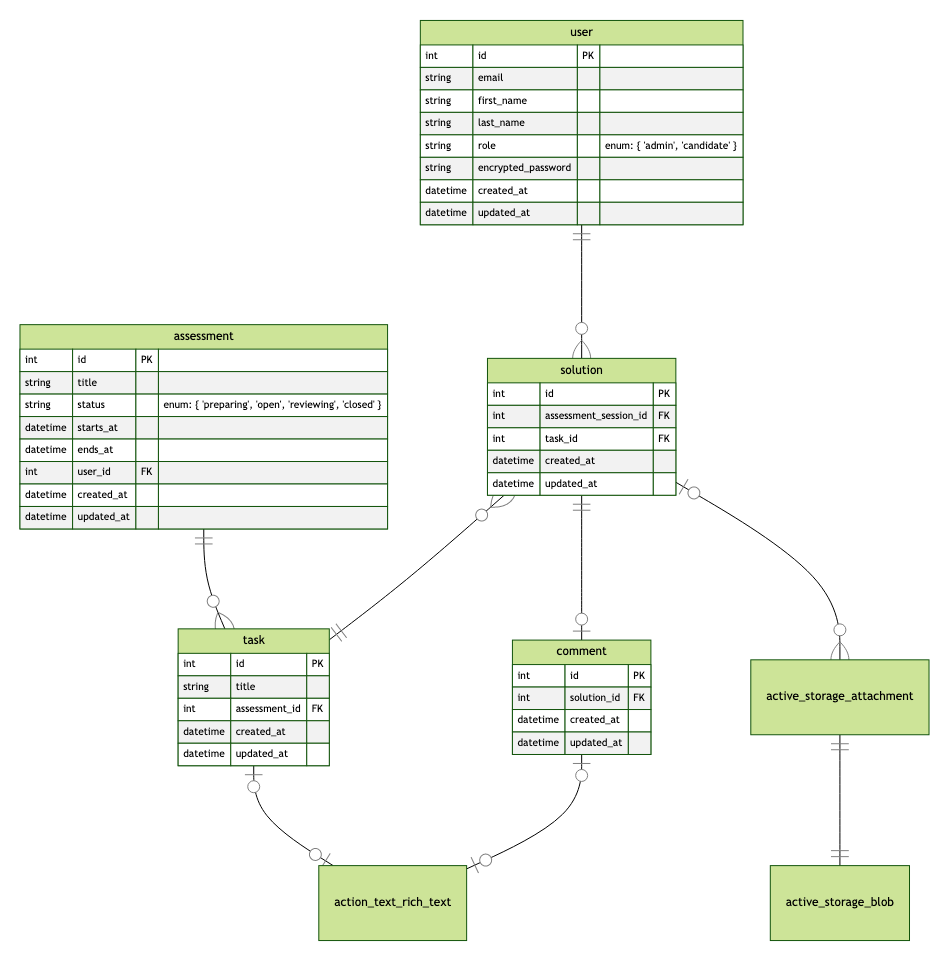
\includegraphics[height=15.25cm]{images/diagrams/entity-relation.png}
    \caption{\label{fig:erd}Entity-relationship Diagramm}
\end{figure}

\newpage

Die drei Entitäten \emph{active\_storage\_attachment}, \emph{active\_storage\_blob} und \emph{action\_text\_rich\_text} werden automatisch durch das
Framework generiert und sollen in diesem Diagramm zum besseren Verständnis des Gesamtkonzeptes beitragen. In der Praxis wird man mit diesen Tabellen direkt kaum etwas zu tun haben.
Diese werden von den zwei gems ActiveStorage und ActionText verwendet, welche das Einbinden von formatierten Textinhalten und Dateiuploads ermöglichen.

Sowohl der Zustand (State) von einem \emph{assessment} als auch die Benutzerrolle von einem \emph{user} wird in Form von einem \gls{enum} abgebildet. Dabei ist zu beachten, dass es in der Praxis kein Database-Level Enum sein wird,
sondern der Wert in Form eines Strings in der Datenbank gespeichert werden soll. Der Constraint wird dann auf Application-Level durchgesetzt. Das ist ein ActiveRecord Standard und ermöglicht eine höhere Flexibilität und Erweiterbarkeit.
Ausserdem werden nicht alle Akteure aus \ref{tab:participants} in Form von Benutzerrollen in der \emph{user} Entität abgebildet, da die Zwei Akteure \enquote{Betreuer} und \enquote{Korrektor} in der Praxis die gleiche Person sein wird.

\subsection{Physisches Datenmodell (Generation)} \label{subsec:model-generation}

Das Ruby on Rails Framework bietet verschiedenste Command-Line Utilities, mit denen man sich relativ einfach gewisse
Grundstrukturen automatisiert generieren lassen kann. Abgeleitet von \ref{fig:erd} können nun die ganzen Commands aufgestellt werden.
Werden diese ausgeführt, erstellen diese sowohl die dazugehörigen Model-Klassen, als auch alle notwendigen Datenbankmigrationen.

\begin{figure}[H]
\begin{codebox}
\begin{minted}{shell}
rails generate model Assessment title:string status:string starts_at:datetime ends_at:datetime
rails generate model AssessmentSession assessment:references user:references
rails generate model Task title:string body:rich_text assessment:references
rails generate model Solution files:attachments task:references user:references
rails generate model Comment body:rich_text solution:references
\end{minted}
\end{codebox}
\caption{\label{fig:generate-models}Commands für die automatisierte Generation von Model-Klassen}
\end{figure}

Die Assoziationen zwischen den Entitäten werden mit dem \emph{references} Typ bereits bei der Generation abgebildet, wodurch
automatisch die Fremdschlüssel erstellt werden. Bei dem \emph{rich\_text} Feldtyp handelt es sich um die bereits angesprochenen formatierten Textinhalte,
welche automatisch in eine andere Tabelle ausgelagert werden. Bei einem \emph{attachment} handelt es sich um einen anhängenden File-Upload.

\newpage

\section{Zustandsdiagramm}

Während dem Lebenszyklus von einem \emph{assessment} durchläuft dieses mehrere Zustände. Diese ändern
sich durch Interaktionen gewisser Akteure mit dem System. Der Zustand verläuft relativ linear von einem Zustand zum nächsten und es gibt keine Abzweigungen
oder sonstige Sonderfälle. Auch eine \enquote{Rückwärtsbewegung} ist ausgeschlossen. Das Diagramm \ref{fig:state-diagram} versucht diesen Prozess zu veranschaulichen.

\begin{figure}[H]
    \centering
    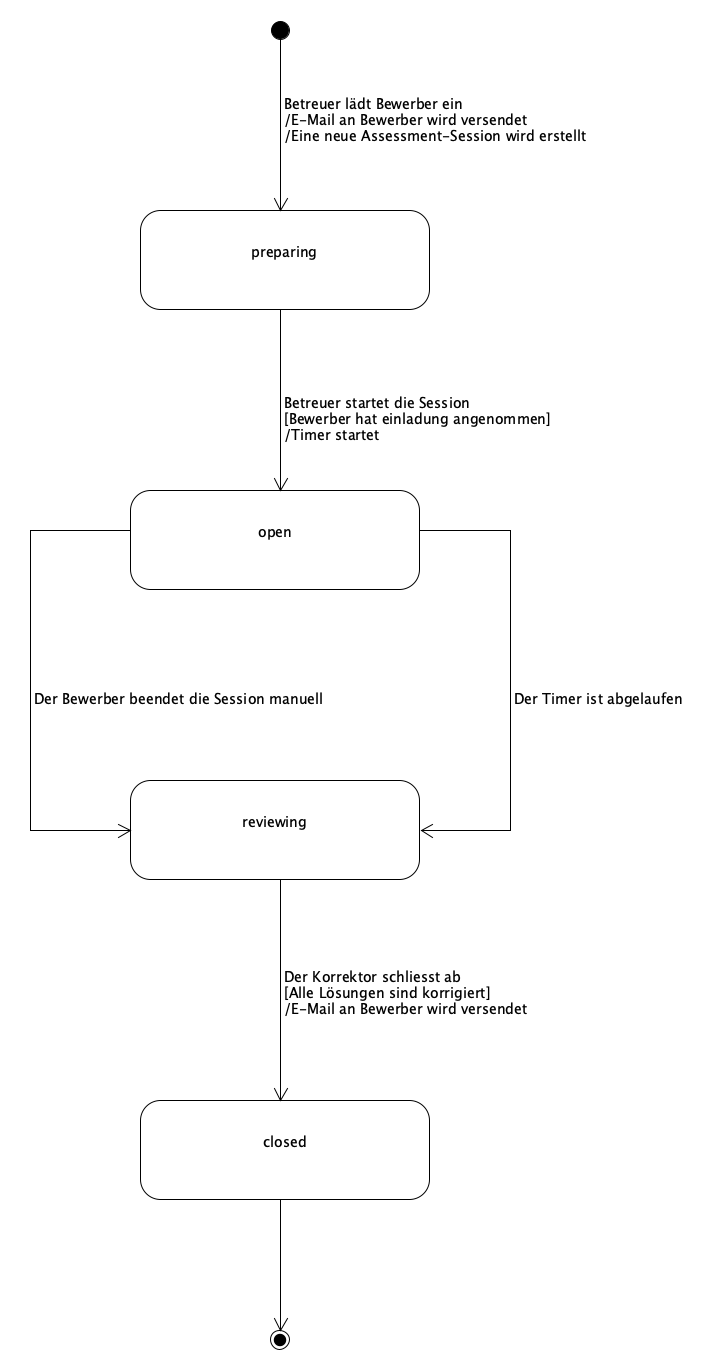
\includegraphics[height=17cm]{images/diagrams/state.png}
    \caption{\label{fig:state-diagram}Zustandsdiagramm eines Assessments nach UML 2.0}
\end{figure}

\newpage

\section{Mockups}

In diesem Abschnitt folgen grobe Entwürfe der verschiedenen Ansichten der Applikation. Diese sollen die Realisierung
erheblich vereinfachen und verschaffen nicht nur einen Überblick über das UI-Design, sondern auch über die genaueren
Funktionalitäten und Benutzer-Flows der Applikation. Die Entwürfe wurden ausserdem nach den Akteuren \ref{tab:participants} kategorisiert.

Bei den Designentwürfen wurde darauf geachtet, diese möglichst minimalistisch zu halten und strikt der Aufgabenstellung zu folgen.
Es wurden keine überflüssigen Elemente eingebaut, um sowohl die Realisierung als auch die spätere Nutzung der Applikation zu vereinfachen.

Ausserdem soll das UI, wie auch schon in den Entwürfen gezeigt wird, vorerst in Englisch umgesetzt werden, da die  offizielle Firmensprache
in der Renuo AG Englisch ist.

\subsection{Bewerber}
\begin{figure}[H]
    \centering
    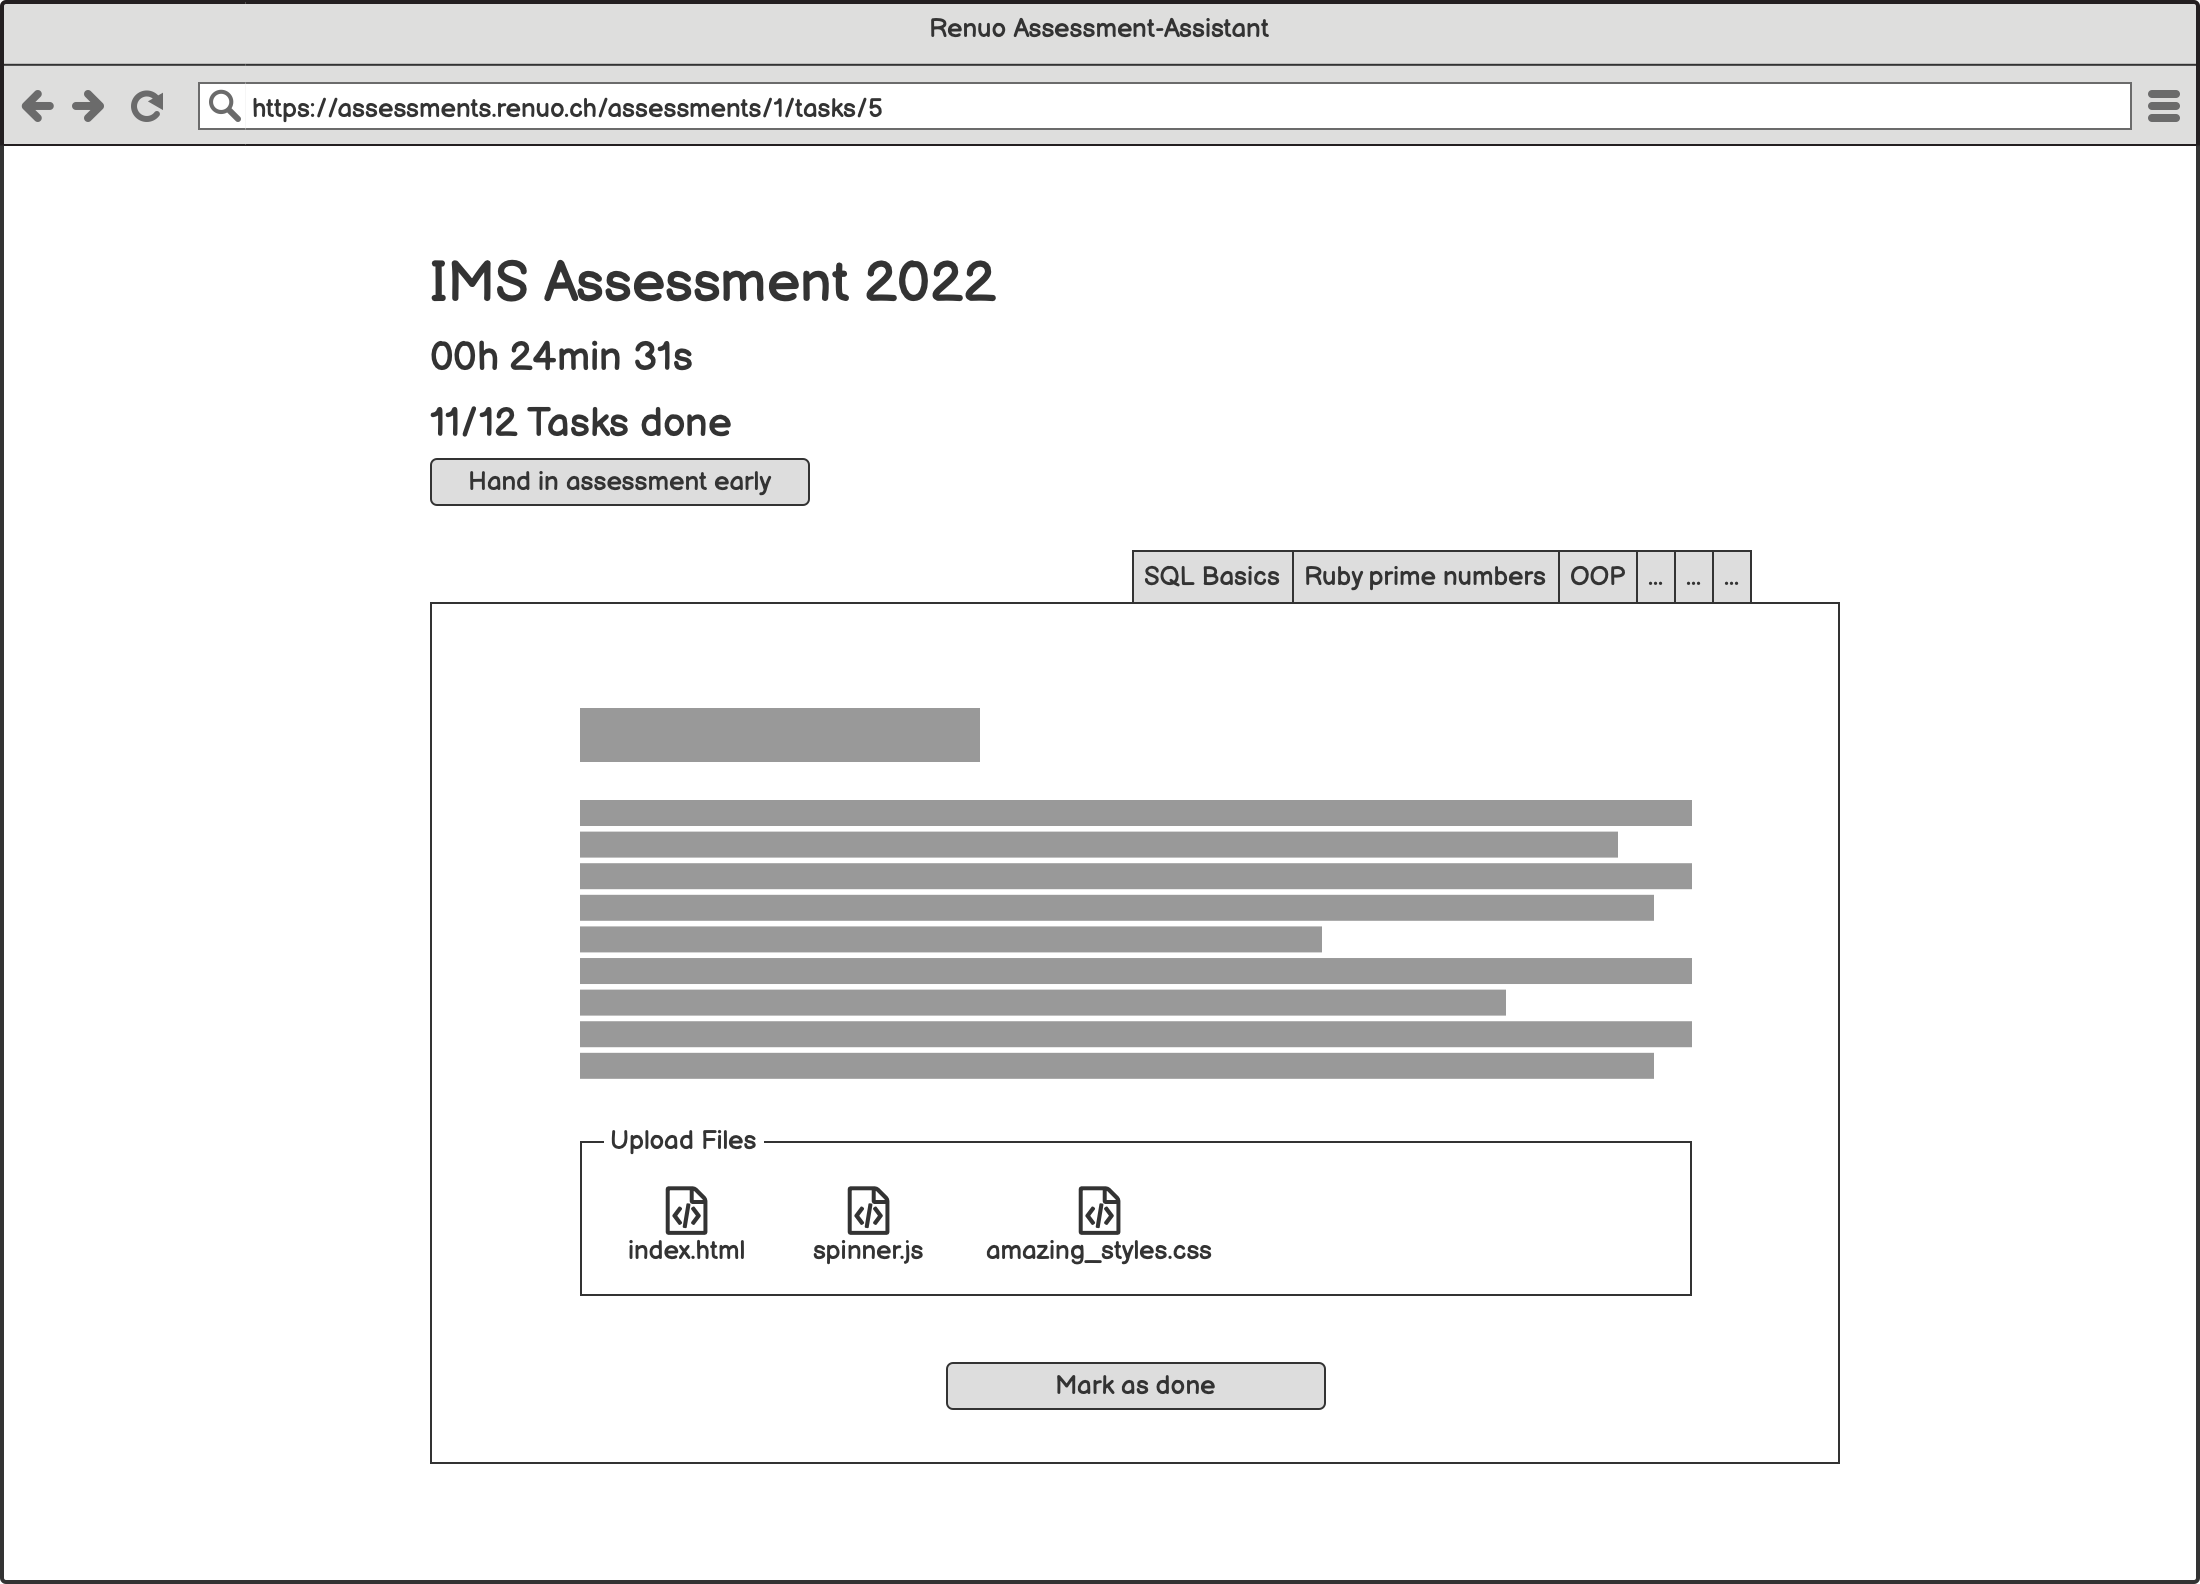
\includegraphics[width=12cm]{images/mockups/candidate-solve-assessment.png}
    \caption{\label{fig:mockup-candidate-solve-assessment}Entwurf für das Lösen eines Assessments}
\end{figure}

\subsection{Betreuer}
\begin{figure}[H]
    \centering
    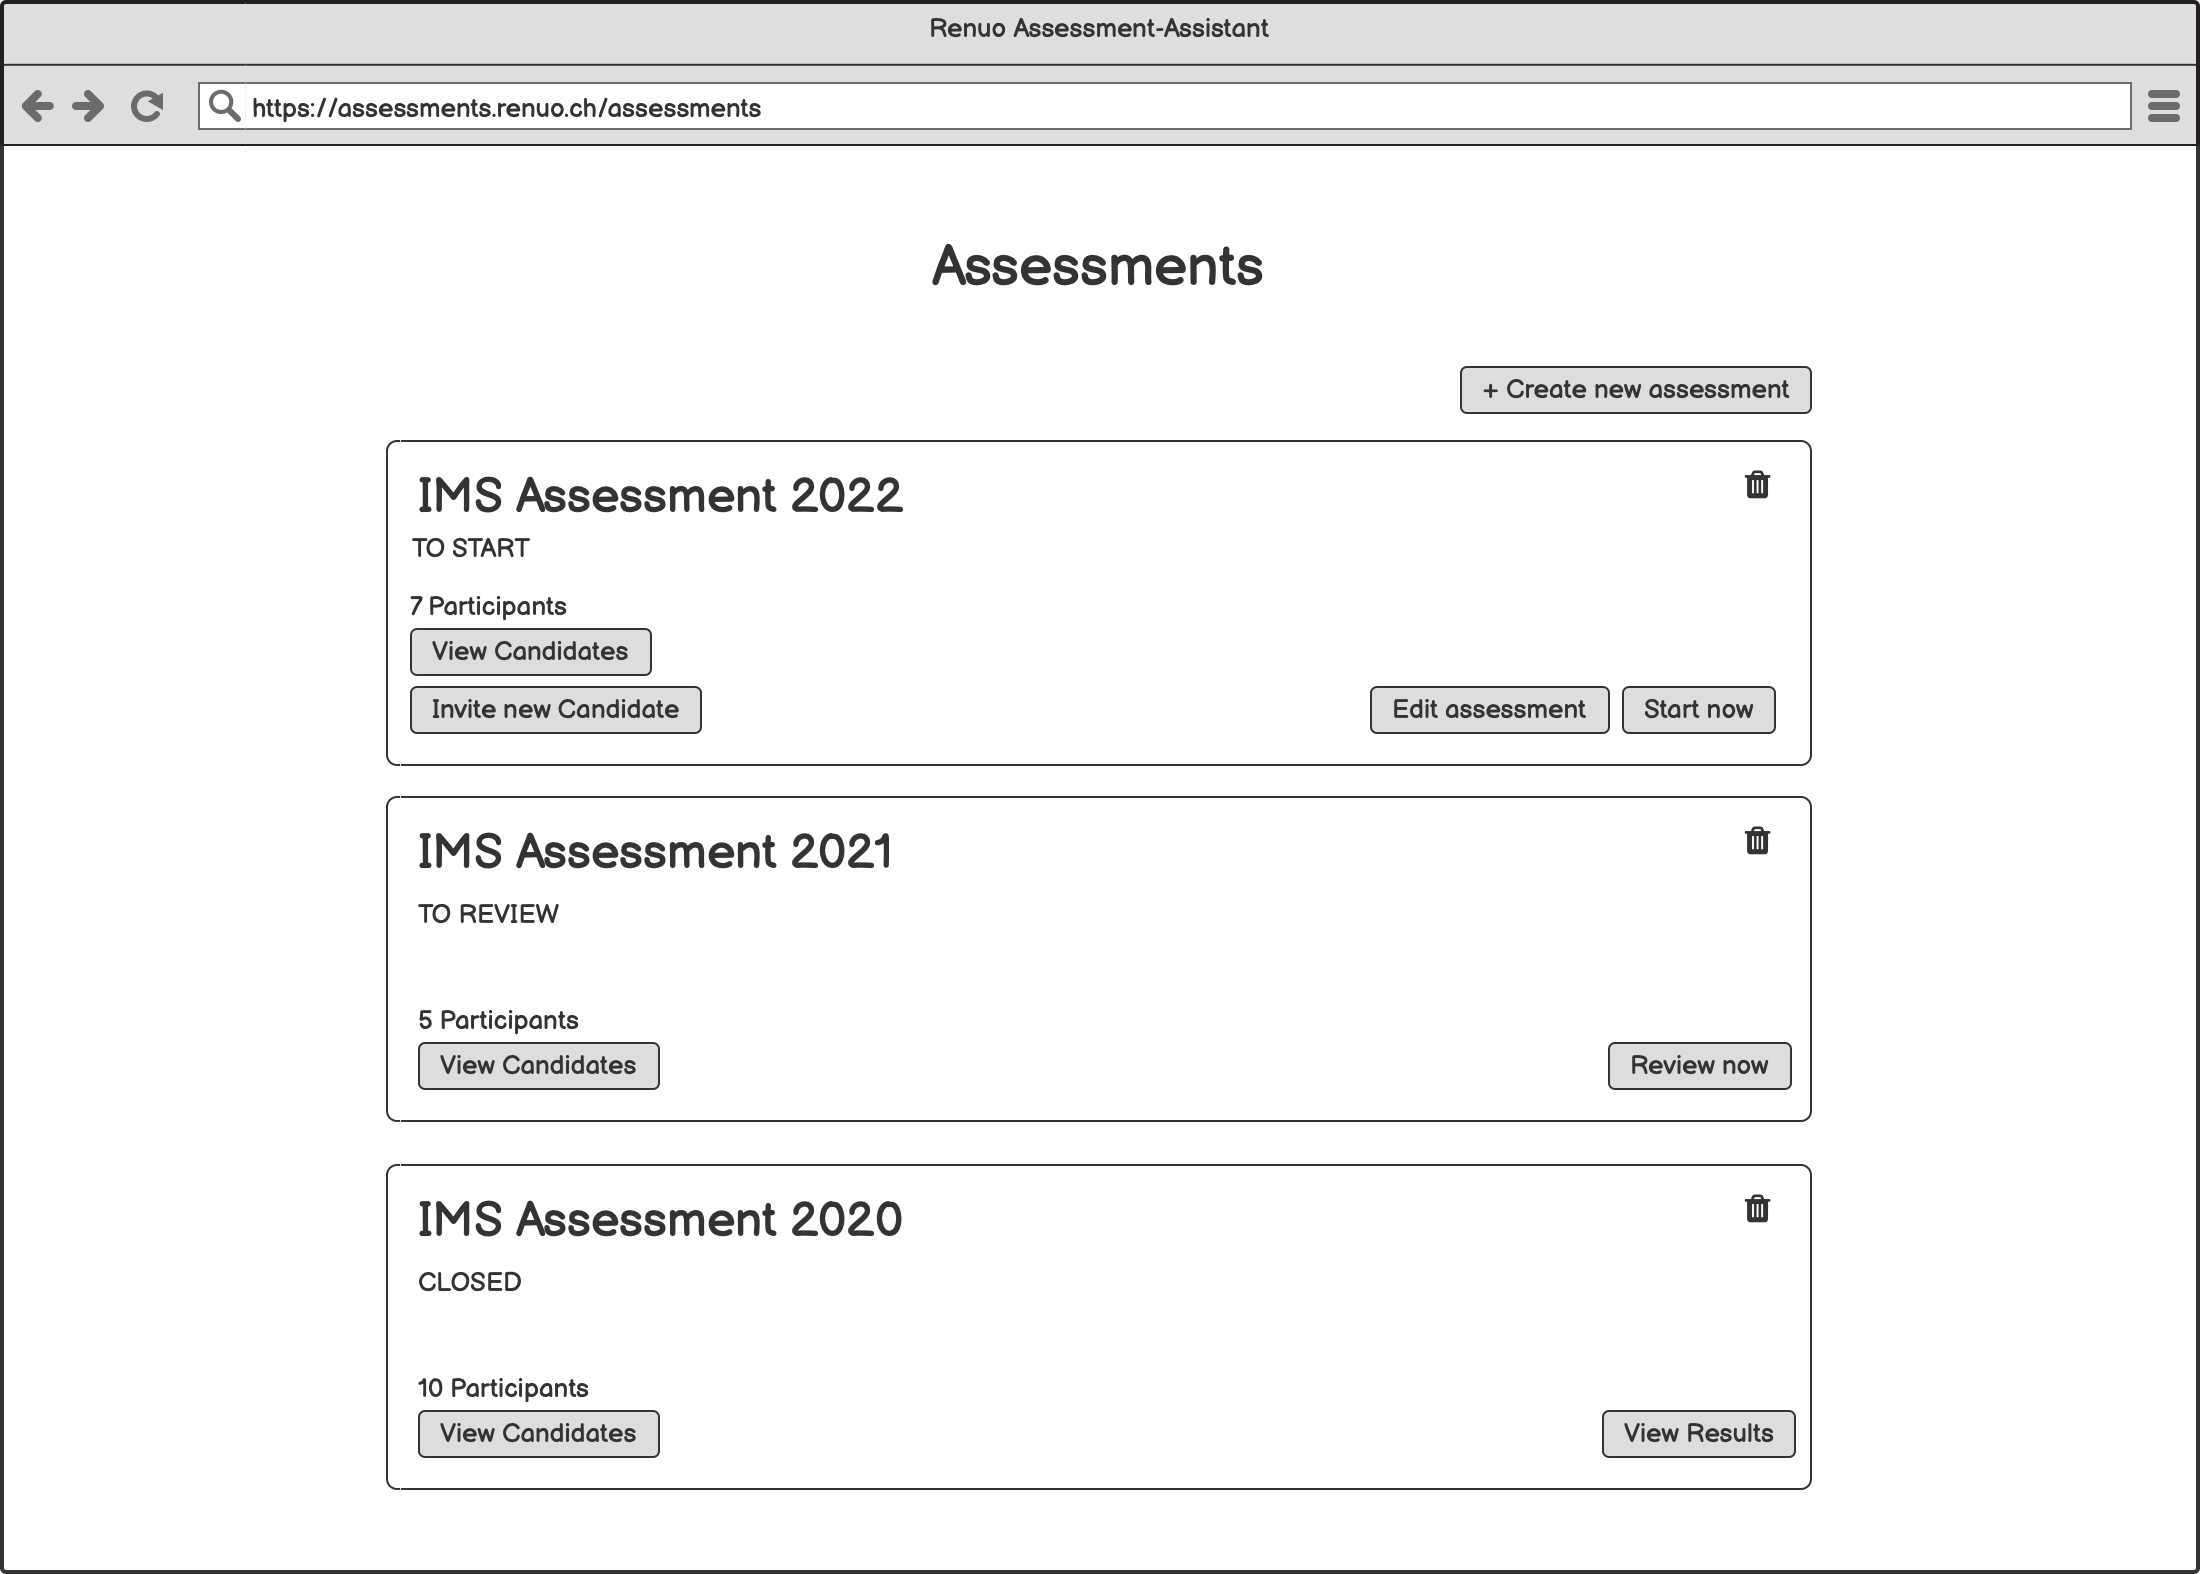
\includegraphics[width=12cm]{images/mockups/supervisor-list-assessments.png}
    \caption{\label{fig:mockup-supervisor-list-assessments}Entwurf für das Auflisten von Assessments}
\end{figure}
\begin{figure}[H]
    \centering
    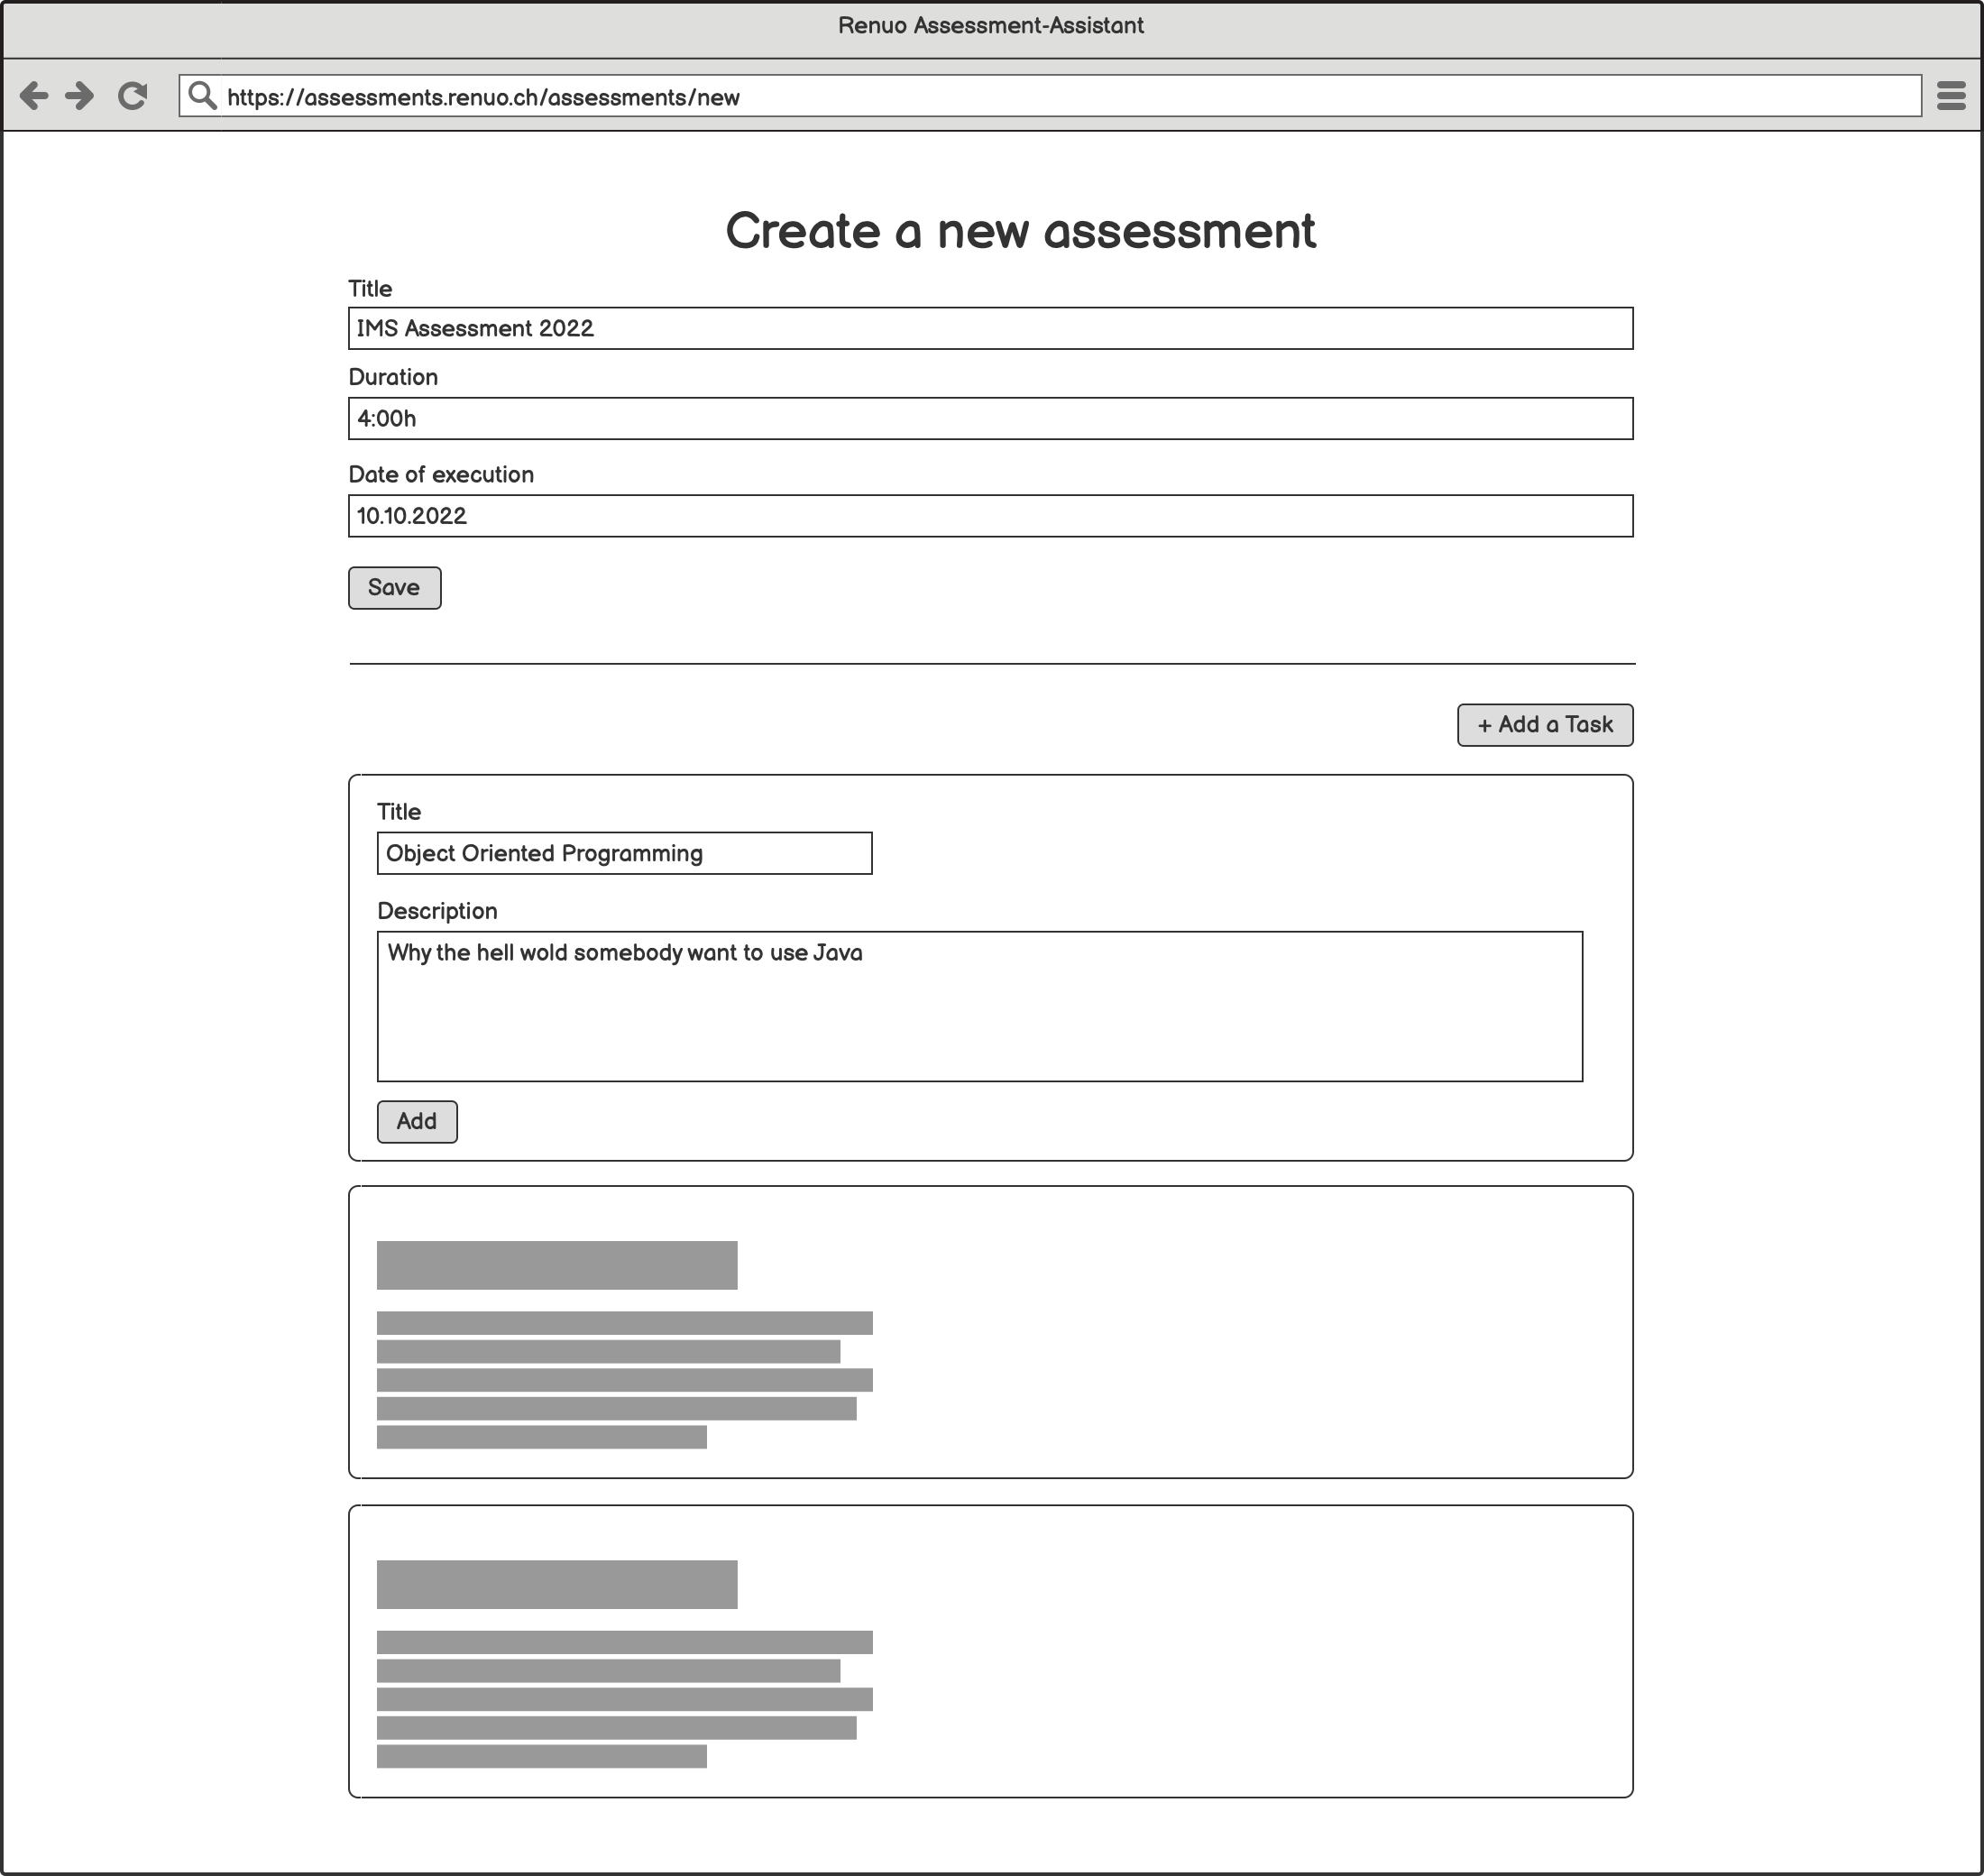
\includegraphics[width=12cm]{images/mockups/supervisor-create-assessment.png}
    \caption{\label{fig:mockup-supervisor-create-assessment}Entwurf für das Erstellen eines neuen Assessments}
\end{figure}

\subsection{Korrektor}
\begin{figure}[H]
    \centering
    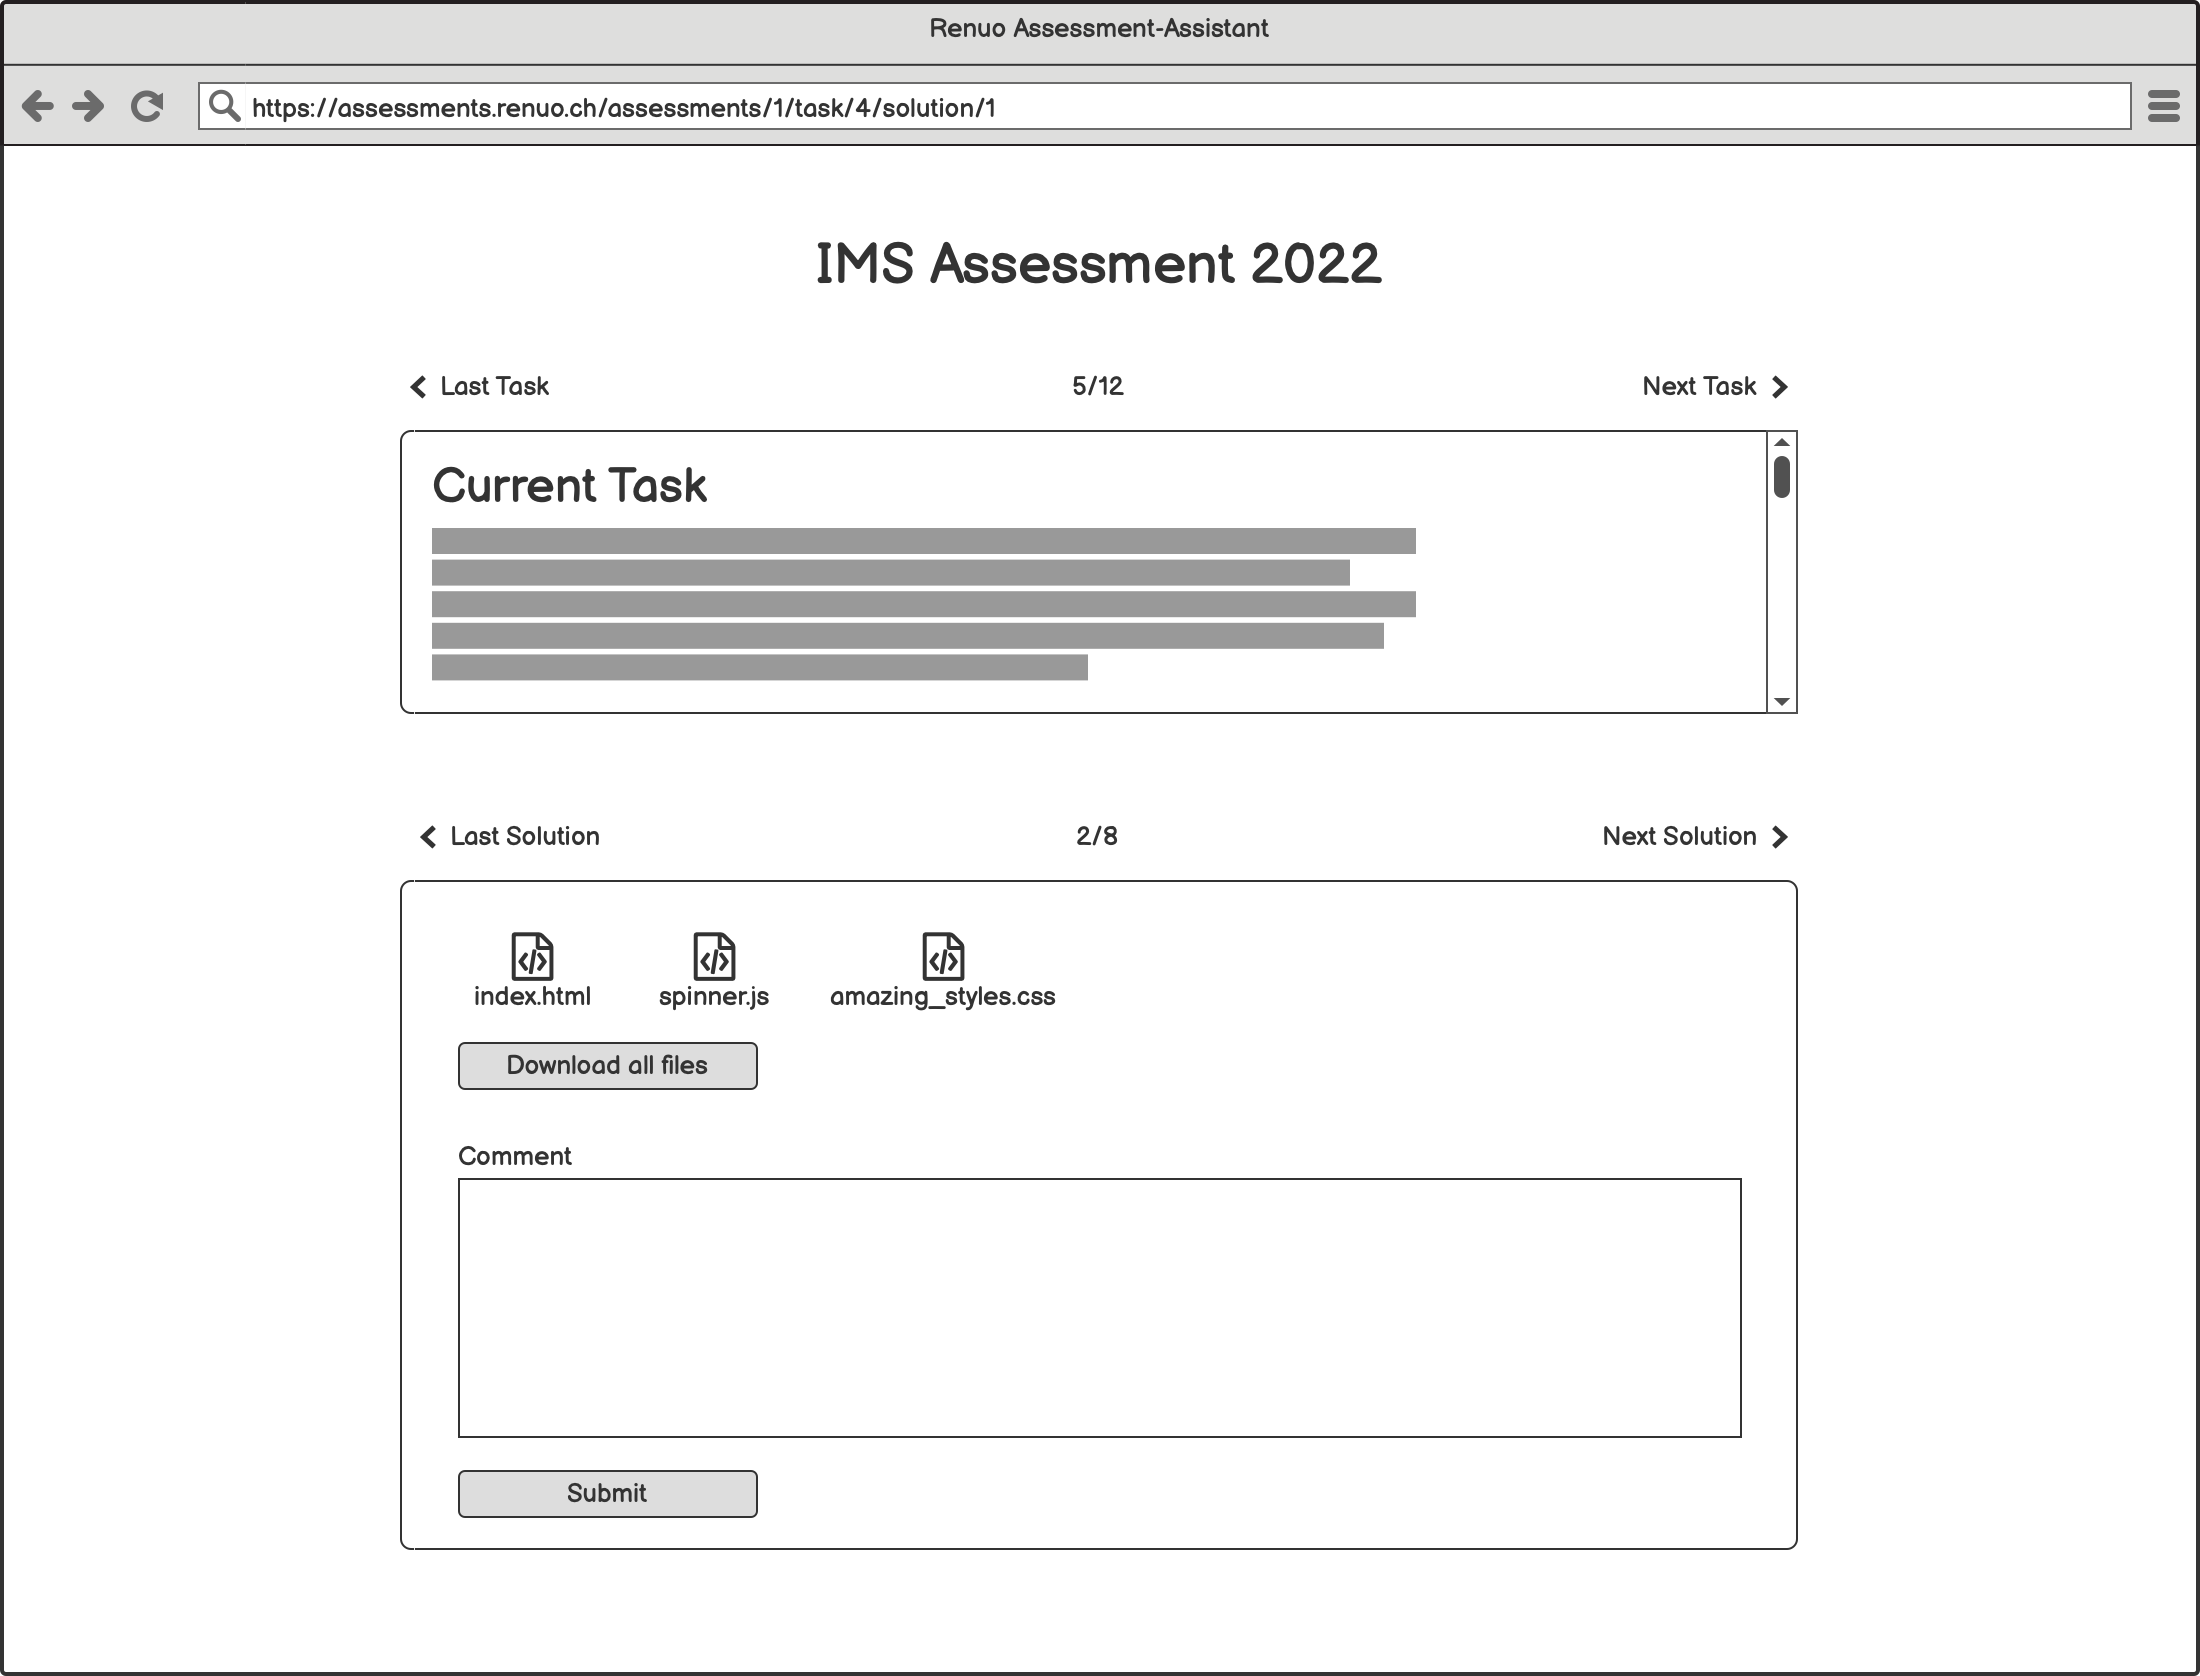
\includegraphics[width=12cm]{images/mockups/corrector-correct-assessment.png}
    \caption{\label{fig:mockup-solve-assessment}Entwurf für das Korrigieren eines Assessments}
\end{figure}
\begin{figure}[H]
    \centering
    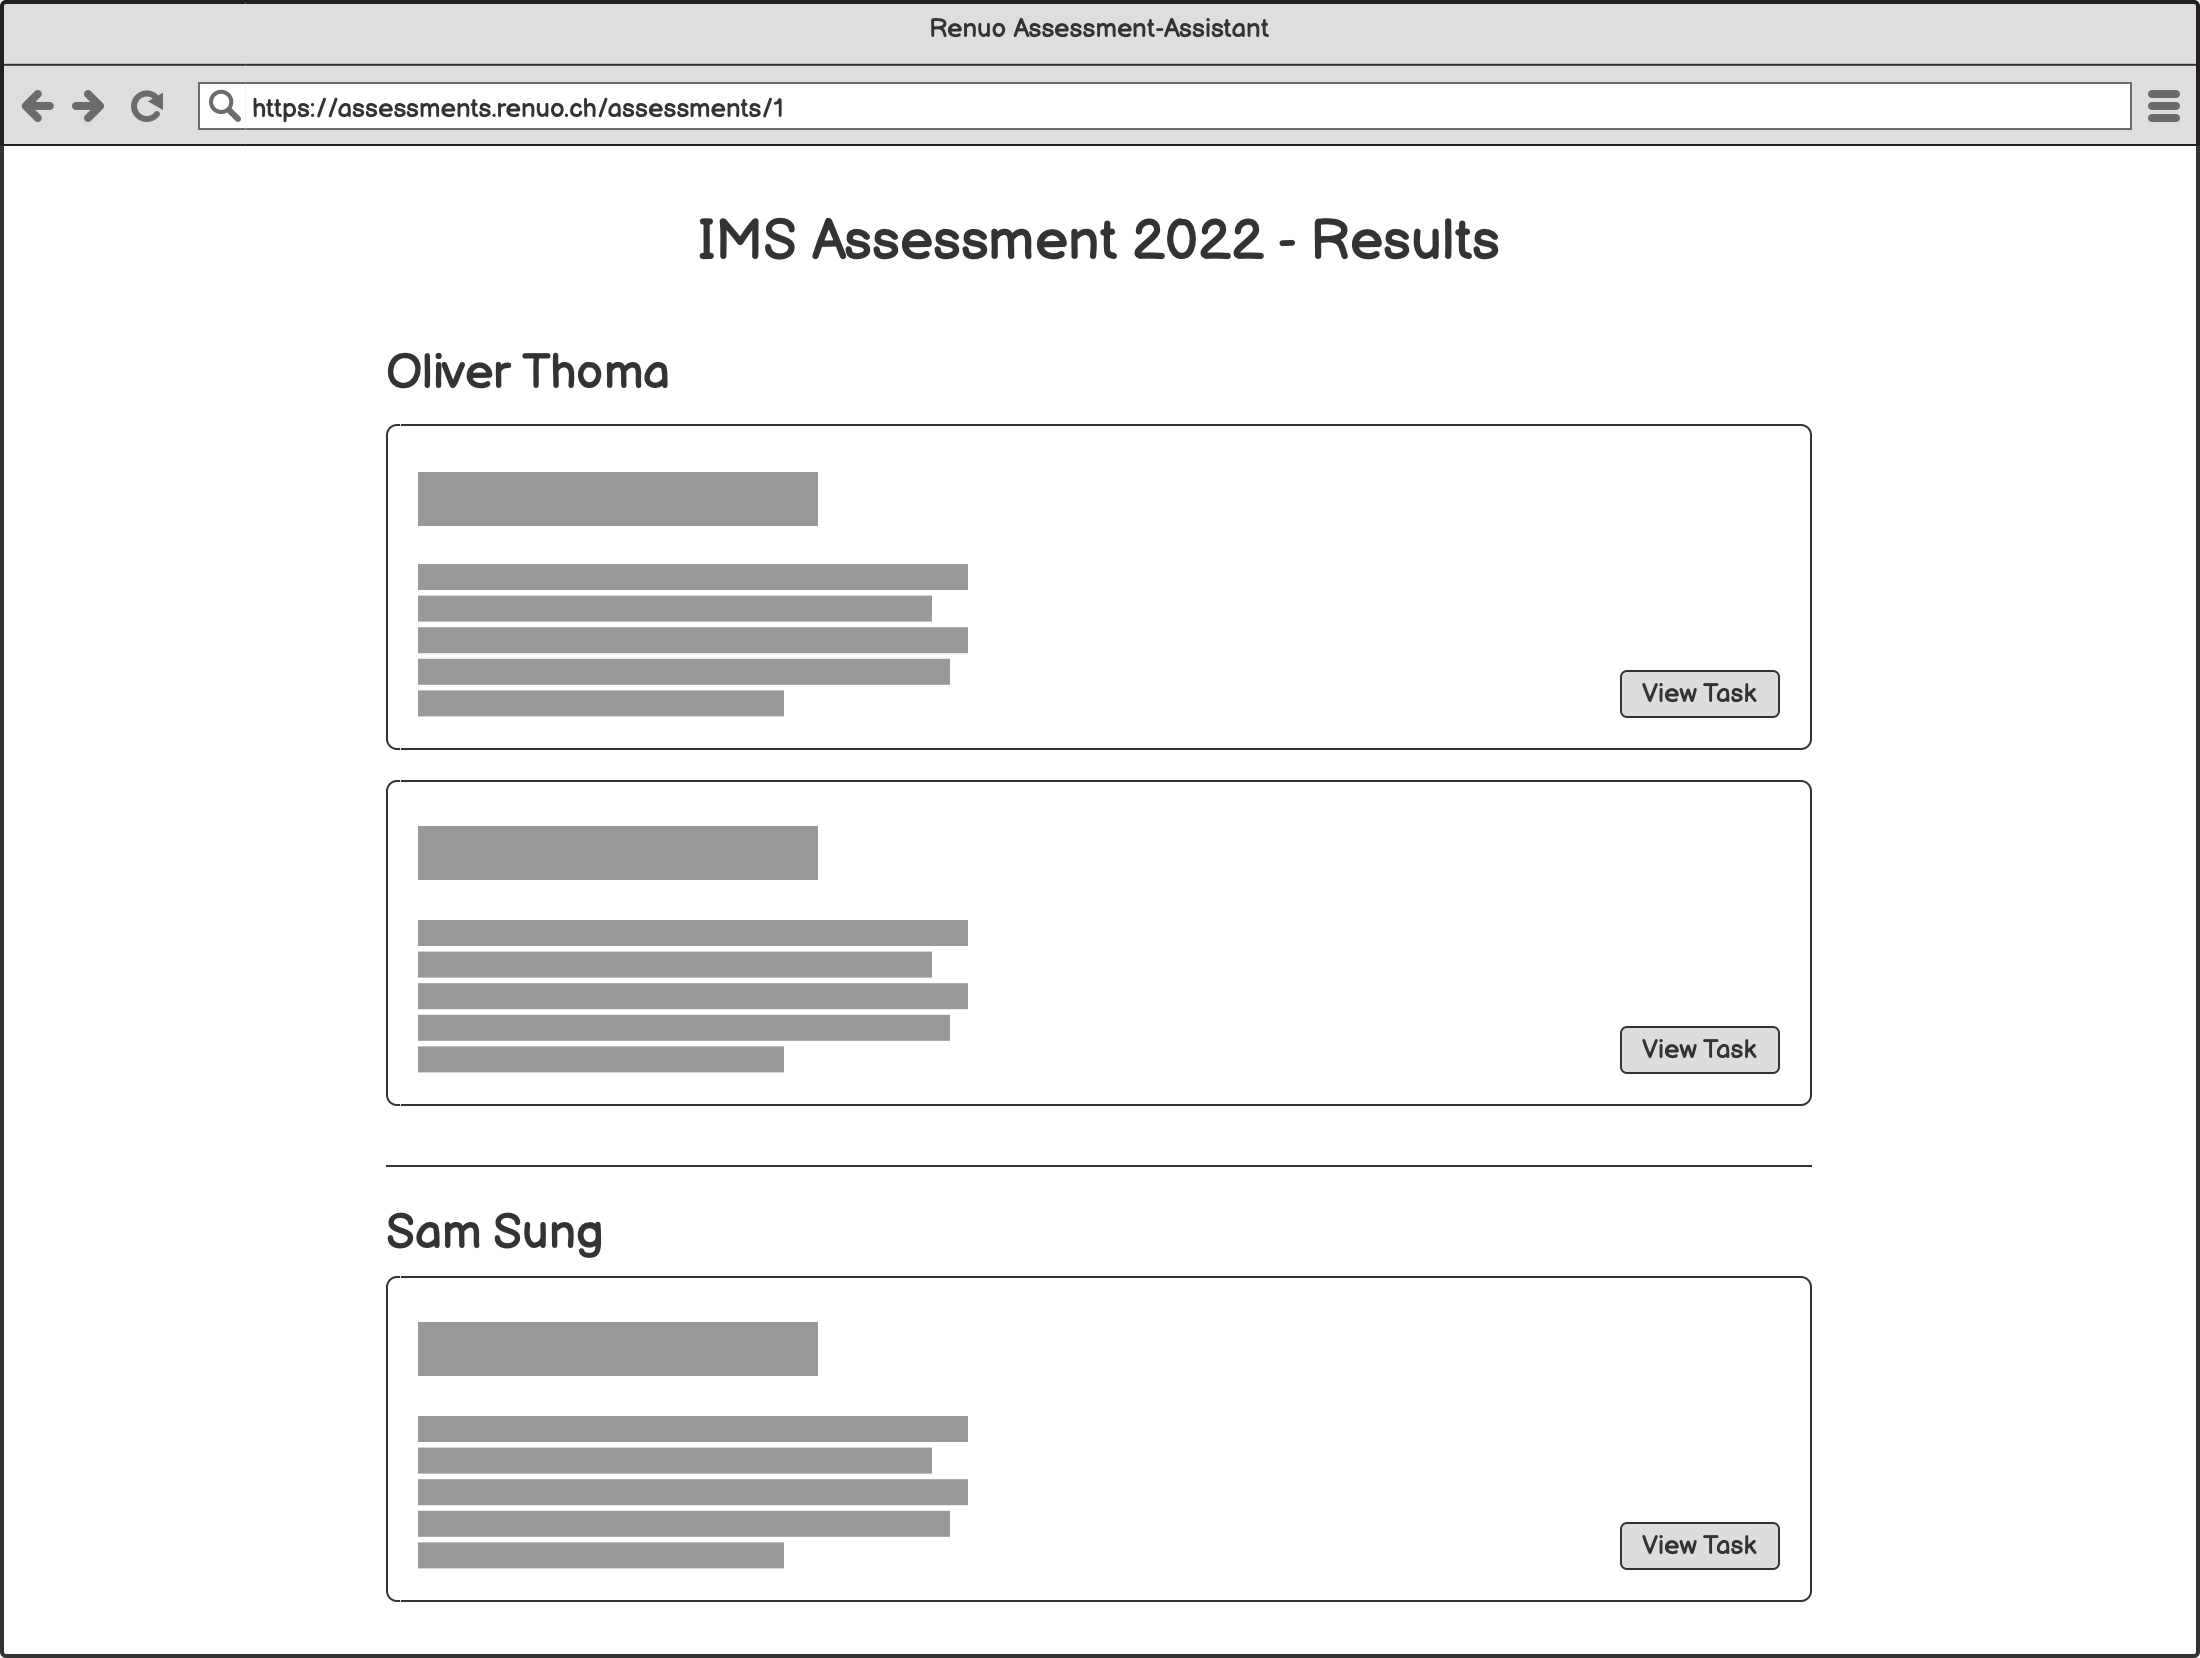
\includegraphics[width=12cm]{images/mockups/assessment-results.png}
    \caption{\label{fig:mockup-assessment-results}Entwurf für das Einsehen und Auflisten der Korrekturen}
\end{figure}

\newpage

\section{Testkonzept} \label{sec:test-concept}

Das Testkonzept beschreibt, wie und mit welchen Werkzeugen das Resultat auf seine Richtigkeit kontrolliert wird.

\subsection{Automatisierte Tests}

Grundsätzlich wird versucht eine Testabdeckung von 100\% durch automatisierte Tests zu erreichen. Die einzelnen
Ziele/Meilensteine der Realisierungsphase werden in dieser PA testgetrieben implementiert. Das heisst, es werden zu Beginn
Unit- und Integrationstests geschrieben und erst dann wird die eigentliche Funktionalität implementiert, bis alle Tests erfolgreich durchlaufen. Dadurch wird
bereits im Voraus über die genauere Implementation nachgedacht und es garantiert immer eine vollständige Testabdeckung.

Bei jedem push auf das Git Repository wird der Code die CI/CD Pipelines auf einer modernen Linux-Umgebung durchlaufen.

Als Testmittel werden ausserdem folgende Softwarebibliotheken eingesetzt:
\begin{itemize}
    \item RSpec
    \item Capybara
    \item FactoryBot
    \item Faker
\end{itemize}

Das Framework benutzt standardmässig eine dedizierte Testdatenbank, die nach jedem Test gereinigt wird. So gibt es keine Abhängigkeiten
oder Konflikte unter einzelnen automatisierten Tests. Die zwei gems \emph{FactoryBot} und \emph{Faker} ermöglichen ausserdem möglichst
realitätsnahe und konsistente Testdaten- und Strukturen.

\subsubsection{Unit Tests}
Alle Model-, Helper- und Service-Klassen werden mittels RSpec Unit-Tests getestet. Diese sollen überprüfen,
ob die einzelnen Komponenten so Arbeiten, wie diese es beabsichtigen.

\subsubsection{Integration Tests}
Die Controller werden per RSpec Integration-Tests getestet. So werden alle Komponenten im Stack der Applikation von ganz oben
nach ganz unten getestet und es wird eine korrekte Integration der darunterliegenden Komponenten sichergestellt.

\subsubsection{System Tests}
Für die einzelnen Benutzer-Flows aller Akteure werden System Tests mit Capybara geschrieben.
Diese öffnen einen headless Chromium Webbrowser und klicken sich automatisiert durch eine im Voraus definierte Sequenz durch.
Dabei werden keine Sonderfälle, sondern lediglich die \gls{happypath} getestet, da die restlichen Sonderfälle wie z.B. Validierungen bereits durch andere Tests gedeckt sind.

\newpage

\subsection{Manuelle Tests}

Die automatisierten Tests decken bereits die wichtigsten Funktionalitäten ab,
jedoch gibt es dennoch Teile in der Applikation, die nur im Kontext des Gesamtsystems getestet werden können.

Die folgenden Tests sollen demnach die vollständige und korrekte Integration der Ruby on Rails Applikation in die Produktions-Umgebung sicherstellen.
Diese werden manuell in einem Web-Browser auf der lokalen Umgebung des Kandidaten ausgeführt, welche in \ref{sec:tools} beschrieben wird.

\subsubsection{Integration von ActiveStorage mit Amazon S3}
\begin{tabularx}{\textwidth}[H]{|s|X|}
    \hline
    ID                  & 1 \\
    \hline

    Beschreibung        &
    Upload und Download von Dateien in realistischen Grössen (etwa 250MB) funktionieren ordnungsgemäss
    \\ \hline

    Vorraussetzung      &
    \begin{itemize}
        \item Einige geeignete Dateien für den Upload wurden vorbereitet
        \item Ein Assessment wurde für diesen Test erstellt und ein Bewerber wurde eingeladen
        \item Man ist eingeloggt mit einem \enquote{Bewerber} Account
    \end{itemize}
    \\ \hline

    Schritte            &
    \begin{itemize}
        \item Das Assessment, zu dem der Bewerber eingeladen wurde, starten und öffnen
        \item Im ersten Task die Datei hochladen
        \item Das Assessment frühzeitig abgeben
        \item Ausloggen und mit einem \enquote{Korrektor} Account einloggen
        \item In die Korrekturansicht wechseln und die Datei herunterladen
    \end{itemize}
    \\ \hline

    Erwartetes Ergebnis &
    Der Bewerber kann die Datei problemlos hochladen und der Korrektor kann diese im ganzen Umfang herunterladen und einsehen.
    \\ \hline
\end{tabularx}

\subsubsection{Integration mit dem Sparkpost E-Mail Service}
\begin{tabularx}{\textwidth}[H]{|s|X|}
    \hline
    ID                  & 2 \\
    \hline

    Beschreibung        &
    E-Mail Benachrichtigungen werden versendet
    \\ \hline

    Vorraussetzung      &
    \begin{itemize}
        \item Es besteht eine E-Mail-Adresse, auf die man Zugriff hat
        \item Es besteht ein \enquote{Betreuer} Account, mit dem bereits ein Assessment für diesen Test erstellt wurde
        \item Man ist eingeloggt mit einem \enquote{Betreuer} Account
    \end{itemize}
    \\ \hline

    Schritte            &
    \begin{itemize}
        \item Auf die Übersichtsseite der Assessments navigieren
        \item Einen neuen Bewerber zu diesem Assessment einladen - mit der vorbereiteten E-Mail-Adresse
    \end{itemize}
    \\ \hline

    Erwartetes Ergebnis &
    Der Bewerber erhält eine Benachrichtigung in sein E-Mail-Postfach, dass er zu einem Assessment bei der Renuo AG eingeladen wurde.
    \\ \hline
\end{tabularx}

\subsubsection{Integration von Hintergrundprozessen mit Heroku-Redis}
\begin{tabularx}{\textwidth}[H]{|s|X|}
    \hline
    ID                  & 3                                                                                        \\
    \hline

    Beschreibung        &
    Der Hintergrundprozess für das rechtzeitige Beenden eines Assessments wird korrekt ausgeführt
    \\ \hline

    Vorraussetzung      &
    \begin{itemize}
        \item Es besteht ein \enquote{Betreuer} Account, mit dem bereits ein Assessment für diesen Test erstellt wurde.
              Dabei sollte die Zeit des Assessments relativ niedrig gesetzt werden.
        \item Es besteht ein \enquote{Bewerber} Account, der bereits in das Assessment eingeladen wurde.
    \end{itemize} \\ \hline

    Schritte            &
    \begin{itemize}
        \item Das Assessment manuell über den \enquote{Betreuer} Account starten.
        \item Mit \enquote{Bewerber} Account einloggen und auf die Aufgabenübersicht wechseln. Dort bleiben, bis der Timer abläuft.
    \end{itemize}
    \\ \hline

    Erwartetes Ergebnis &
    Ein Beenden des Assessments wird nach Ablauf der Zeit erzwungen und dessen Status ändert sich zu \enquote{Reviewing}.
    \\ \hline
\end{tabularx}

\chapter{Entscheiden} \label{ch:decide}

Die meisten Entscheidungen bezogen auf das Gesamtsystem und die zu verwendenden Softwarebibliotheken werden bereits durch das
\emph{Renuo Application-Setup-Guide} abgenommen. Dennoch gibt es verschiedene Varianten von Softwarebibliotheken und Konzepten,
zwischen denen in diesem Kapitel möglichst objektiv entschieden werden soll. Dazu werden simple Nutzwertanalysen eingesetzt.

Diese Nutzwertanalysen vergleichen die vorliegenden Varianten basierend auf 6 Kriterien, welche anhand eines Punktesystems mit jeweils 0 bis 5 Punkten bewertet werden.
Jedes dieser Kriterien hat eine andere Gewichtung, bezogen auf deren Wichtigkeit in der Umsetzung dieser PA.
Dabei spielen die bestehenden Kenntnisse des Kandidaten über die einzelnen Varianten eine sehr grosse Rolle,
da das Projekt in einer sehr kurzen Zeit umgesetzt werden soll und werden daher besonders stark gewichtet.

\section{State Management}
Um das Verwalten der in dem Diagramm \ref{fig:state-diagram} beschriebenen Zustände eises Assessments zu vereinfachen,
wird das Konzept einer \emph{State-Machine} eingeführt. Eine solche \enquote{Zustandsmaschine} liest eine Reihe von Eingaben
und ändert den Zustand des jeweiligen Assessments bei jeder Eingabe entsprechend. Ausserdem ermöglicht dieses Konzept einen nachvollziehbaren
Fluss und garantiert einen sauberen, lesbaren Code. In der Ruby-Welt gibt es Unmengen an Softwarebibliotheken, die ein solches Konzept implementieren.
Für diesen Entscheid wurden zwei der beliebtesten gems basierend auf deren \enquote{GitHub Stars} ausgewählt.

\subsubsection{Variante 1: \enquote{stateful\_enum}}

Diese Variante ermöglicht eine perfekte Integration in das Framework, indem sie auf der \emph{ActiveRecord::Enum} \gls{dsl} aufbaut und somit eine einfache Syntax bietet.
Es werden \emph{events} definiert, welche Übergänge zwischen Zuständen beschreiben und einen optionalen \emph{before} Callback haben.

\begin{figure}[H]
\begin{codebox}
\begin{minted}{ruby}
class Bug < ApplicationRecord
  enum status: { unassigned: 0, assigned: 1, resolved: 2 } do
    event :assign do
      transition :unassigned => :assigned
    end

    event :resolve do
      before do
        self.resolved_at = Time.zone.now
      end
      transition [:unassigned, :assigned] => :resolved
    end
  end
end
\end{minted}
\end{codebox}
\caption{\label{fig:stateful-enum-example}Beispiel einer Zustandsmaschine mit dem \enquote{stateful\_enum} gem \cite{stateful_enum_github}}
\end{figure}

\subsubsection{Variante 2: \enquote{state\_machines}}

Mit fast 100 Millionen Downloads \cite{statstate_machines-activemodel_rubygems} ist diese Variante bestimmt eine der Bekanntesten Lösungen für Zustandsmaschinen in Ruby.
Das gem ist sehr umfangreich und bietet viele Funktionalitäten in einer eigenen DSL. Es gibt verschiedenste Forks dieses gems,
die auch perfekt mit dem Ruby on Rails Framework integrieren. So gibt es beispielsweise Model-Validierungen über eine \emph{ActiveModel::Validations} Integration,
verschiedenste Arten von Callbacks, parallele Events u.v.m.

\begin{figure}[H]
\begin{codebox}
\begin{minted}{ruby}
class Vehicle
  state_machine :initial => :parked do
    before_transition :parked => any - :parked, :do => :put_on_seatbelt
    after_transition any => :parked do |vehicle, transition|
      vehicle.seatbelt = 'off'
    end
    around_transition :benchmark

    event :ignite do
      transition :parked => :idling
    end

    state :first_gear, :second_gear do
      validates_presence_of :seatbelt_on
    end
  end

  ...
end
\end{minted}
\end{codebox}
\caption{\label{fig:state-machine-example}Beispiel einer Zustandsmaschine mit dem \enquote{state\_machines} gem \cite{state_machines-activemodel_github}}
\end{figure}

\subsubsection{Nutzwertanalyse}

Die zwei Varianten unterscheiden sich sehr stark durch den Umfang an Features die sie bieten,
jedoch wird für diese PA nur eine simple Form einer Zustandsmaschine benötigt. Durch die einfach gehaltene Syntax
und die gute Integration in \emph{ActiveRecord::Enum} ist die 1. Variante der klare Gewinner der folgenden Nutzwertanalyse.

\begin{table}[H]
  \rowcolors{2}{gray!10}{white}
  \begin{tabular}{|l|l|l|l|}
    \hline
    \rowcolor{PrimaryColor!30} \textbf{Kriterium} & \textbf{Gewichtung} & \textbf{Variante 1} & \textbf{Variante 2} \\
    \hline
    Kenntnisse                                    & 40 \%               & 1                   & 0                   \\
    \hline
    Dokumentationen/Anleitungen                   & 20 \%               & 5                   & 5                   \\
    \hline
    Komplexität                                   & 10 \%               & 5                   & 2                   \\
    \hline
    Umfang/Features                               & 15 \%               & 2                   & 5                   \\
    \hline
    Integration in das Framework                  & 15 \%               & 5                   & 4                   \\
    \hline
    \hline
    SUMME \emph{inkl. Gewichtung}                 & \textbf{100 \%}     & \textbf{2.95}       & \textbf{2.55}       \\
    \hline
  \end{tabular}
\end{table}

\newpage

\section{Autorisierung} \label{sec:authorization}

Damit ein Benutzer mit der Rolle \enquote{candidate} nur Ressourcen einsehen und bearbeiten kann, zu denen dieser berechtigt ist,
wird ein System für eine Autorisierung benötigt. Diese Autorisierungsbibliothek sollte mit dem Authentifizierungs gem \emph{Devise} kompatibel sein, da dieses in dieser PA eingesetzt wird.
Ausserdem sollte die Implementation möglichst einfach mit den in \ref{} beschriebenen Testmitteln testbar sein.
Auch für diesen Variantenvergleich wurden zwei der beliebtesten Bibliotheken herbeigezogen, welche den genannten Kriterien entsprechen.

\subsubsection{Variante 1: \enquote{CanCanCan}}

Alle Berechtigungen können in \emph{CanCanCan} in einer einzigen \enquote{Fähigkeitsdatei} definiert werden, sodass die Berechtigungslogik für einfache Wartung und Tests an einer Stelle bleibt.
Ausserdem stellt die Bibliothek viele Helper zur Verfügung, um diese Berechtigungen in verschiedensten orten der Applikation abzufragen. Auch wird das Testing mittels \emph{RSpec} durch mitgelieferte \enquote{Matcher} erheblich erleichtert.

\subsubsection{Variante 2: \enquote{Pundit}}

\emph{Pundit} definiert sogenannte \enquote{Policies} für einzelne Ruby-Klassen. Das heisst, es gibt nicht nur eine einzelne \enquote{Fähigkeitsdatei},
sondern die Berechtigungen werden in mehrere Dateien aufgeteilt und explizit für jedes Model definiert. Jedoch können auch globale Policies definiert werden.
Auch stehen zwar sehr ähnliche, jedoch nicht so viele Helper-Klassen zur verfügung wie in dem \emph{CanCanCan} gem. Auch \emph{RSpec Matcher} kommen nicht out-of-the-box mit dem gem mitgeliefert.

\subsubsection{Nutzwertanalyse}

Der Gewinner der folgenden Nutzwertanalyse ist eindeutig die 1. Variante. Die beiden gems unterscheiden sich kaum durch deren Umfang an Features und schlussendlich waren vor allem die Vorkenntnisse
ausschlaggebend für diese Entscheidung. Gearbeitet hat der Kandidat bereits mit beiden gems, jedoch kommt \emph{CanCanCan} in Projekten der Renuo AG wesentlich häufiger zum Einsatz.

\begin{table}[H]
  \rowcolors{2}{gray!10}{white}
  \begin{tabular}{|l|l|l|l|}
    \hline
    \rowcolor{PrimaryColor!30} \textbf{Kriterium} & \textbf{Gewichtung} & \textbf{Variante 1} & \textbf{Variante 2} \\
    \hline
    Kenntnisse                                    & 40 \%               & 5                   & 2                   \\
    \hline
    Dokumentationen/Anleitungen                   & 20 \%               & 5                   & 5                   \\
    \hline
    Komplexität                                   & 10 \%               & 4                   & 3                   \\
    \hline
    Umfang/Features                               & 15 \%               & 3                   & 4                   \\
    \hline
    Integration in das Framework                  & 15 \%               & 5                   & 5                   \\
    \hline
    \hline
    SUMME \emph{inkl. Gewichtung}                 & \textbf{100 \%}     & \textbf{4.6}        & \textbf{3.45}       \\
    \hline
  \end{tabular}
\end{table}

\chapter{Realisieren} \label{ch:implement}

Gestützt auf den vorherigen Phasen der gewählten Projektmanagementmethode wird in diesem Kapitel die eigentliche Implementation des Systems dokumentiert.
Diese soll bezogen auf den Arbeitsprozess möglichst linear wiedergegeben werden.

\section{Versionierung und Backups} \label{sec:backups}

\subsection{Code}

Die Ruby on Rails Applikation wird gemäss Renuo-Guidelines in einem Git-Repository auf GitHub versioniert. Es werden keine Pull Requests erstellt,
da diese für eine Einzelarbeit in dieser Grösse keinen Nutzen von sich tragen. Stattdessen wird versucht, eine möglichst saubere History zu schaffen mit kurzen, aussagekräftigen Git Commit-Messages.
So ist der Verlauf der Arbeit gut nachvollziehbar und es kann jederzeit auf eine vergangene Version zurückgegriffen werden. Nach jedem Commit
wird dieser direkt auf den remote \emph{develop} Branch gepusht.

\begin{figure}[H]
    \centering
    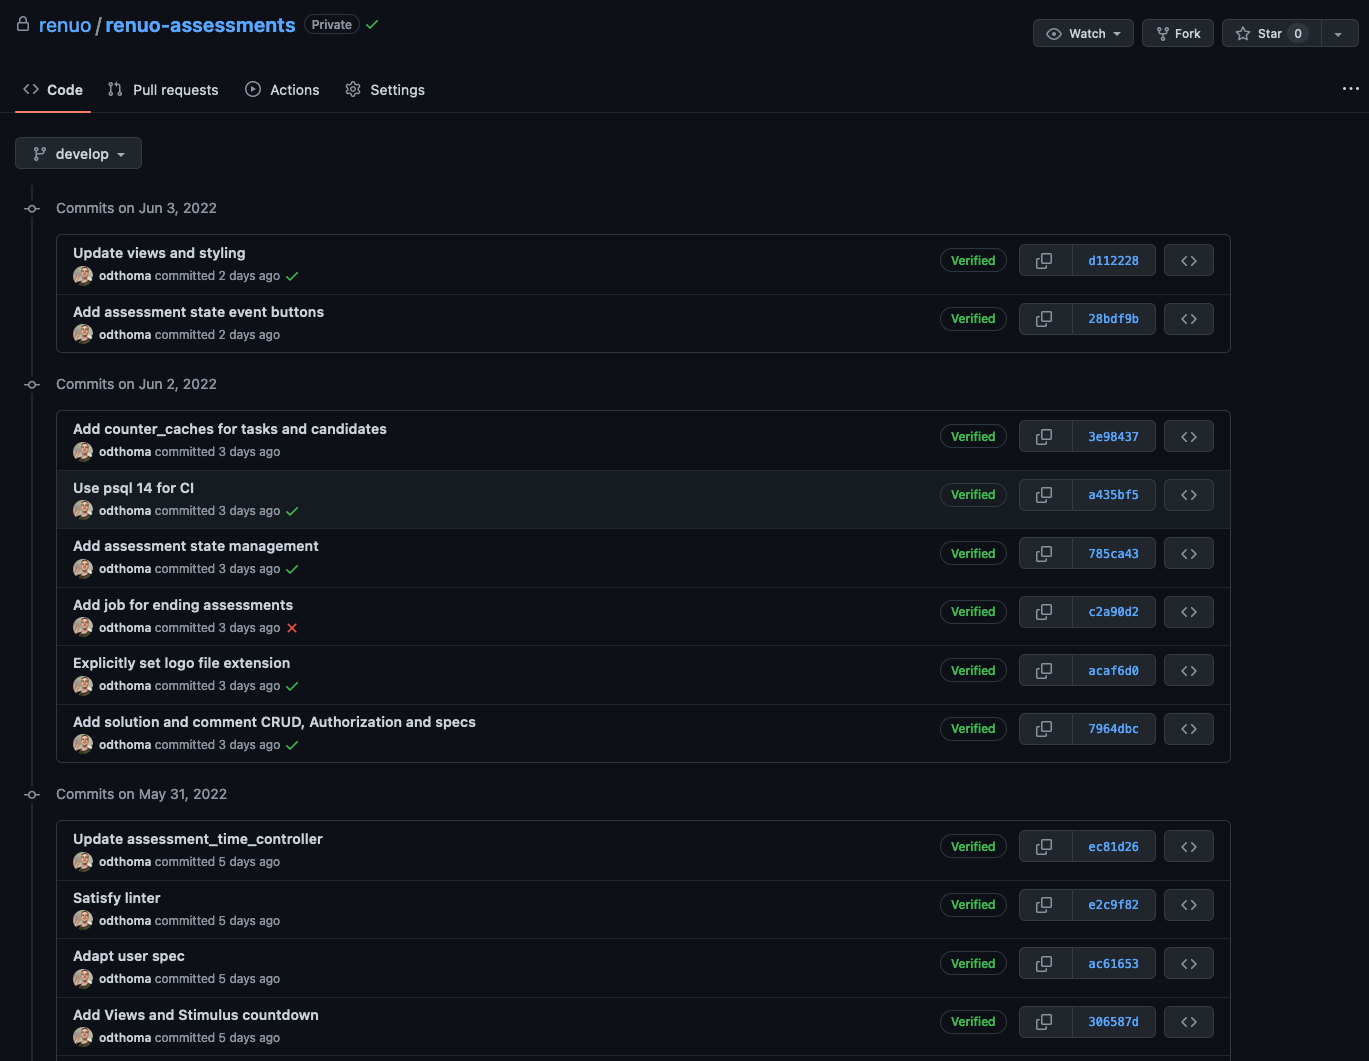
\includegraphics[width=14cm]{images/renuo-assessments-github.png}
    \caption{\label{fig:renuo-assessments-github}Ausschnitt der GitHub Commit-History vom Ruby on Rails Projekt}
\end{figure}

\newpage

\subsection{IPA-Bericht}

Das LaTeX Projekt wird ebenfalls in einem Git-Repository versioniert und es werden zu sinnvollen Zeitpunkten Commit gemacht. Diese werden dann regelmässig auf ein Remote (GitHub) gepusht und es wird jeden Abend ein neuer Git-Tag erstellt.
In dem Repository befinden sich alle Diagramme und sonstigen Dateien, die für die Umsetzung des IPA-Berichtes notwendig sind. 
So ist eine rasche Wiederherstellung der aktuellen Daten im Falle eines Datenverlustes jederzeit und von überall aus möglich.

\begin{figure}[H]
    \centering
    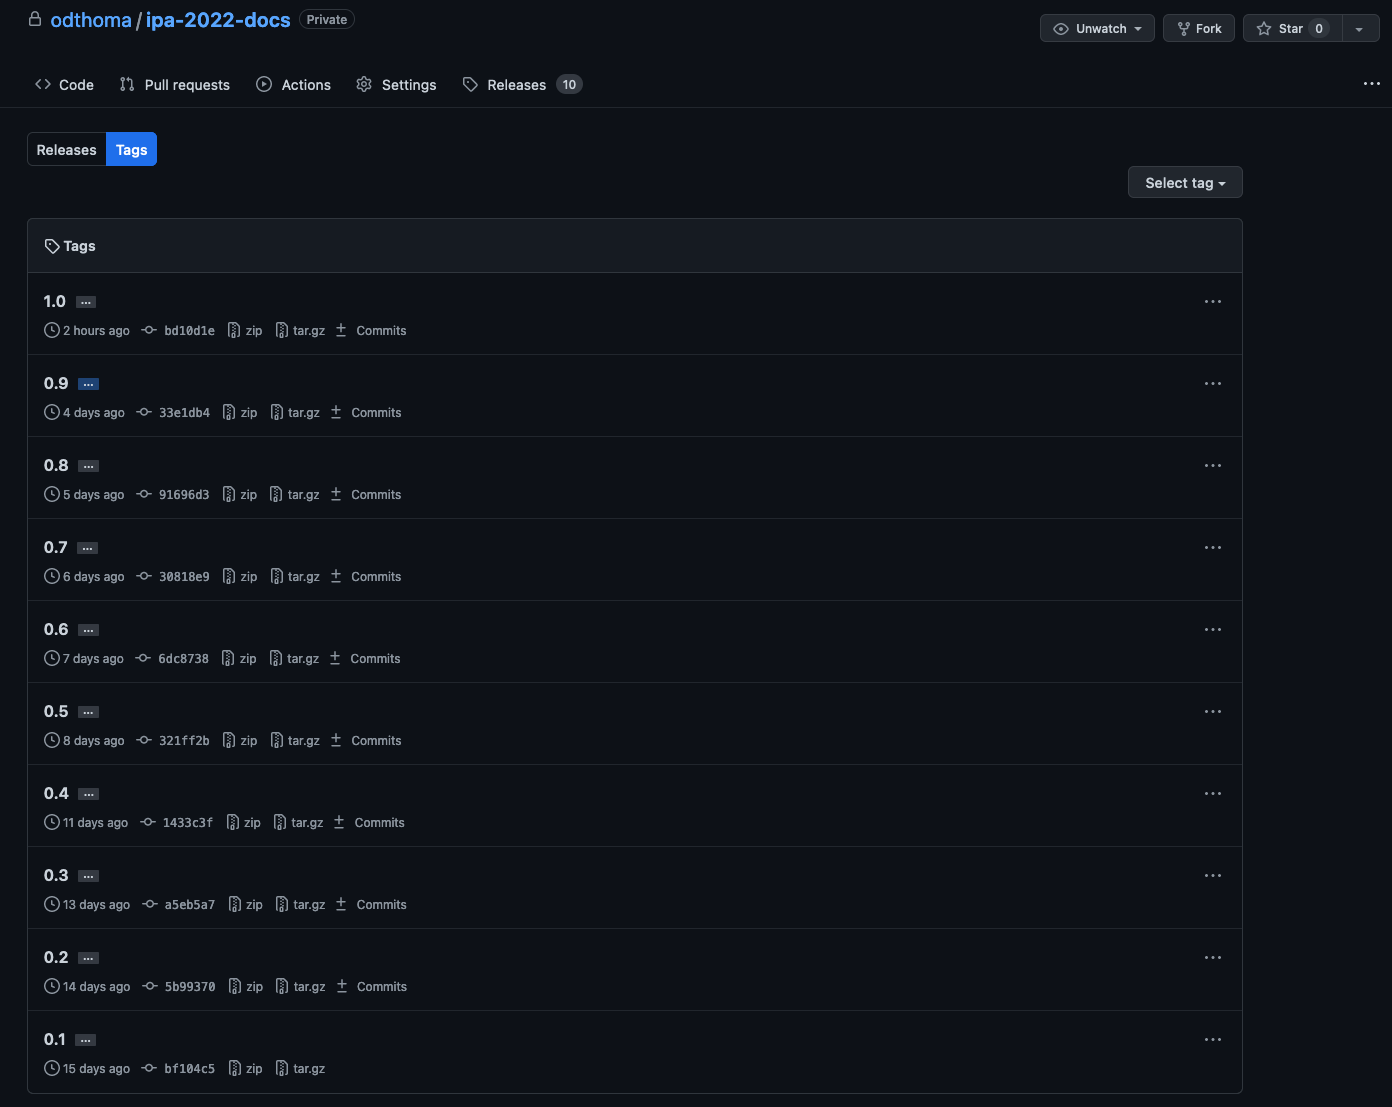
\includegraphics[width=14cm]{images/latex-github-tags.png}
    \caption{\label{fig:latex-github-tags}Tägliche Versionierung des IPA-Berichts über Git-Tags}
\end{figure}


\chapter{Kontrollieren} \label{ch:check}

In diesem Kapitel wird das Endprodukt auf seine Richtigkeit überprüft und alle
Tests werden dem Testkonzept \ref{sec:test-concept} entsprechend ausgeführt, ausgewertet und protokolliert.

\section{Automatisierte Tests}

Es besteht die geforderte Testabdeckung von 100\% und es wurden in der Realisierungsphase, wie geplant, laufend neue Unit- und Integrationtests geschrieben.
Diese wurden jeweils so aufgestellt, dass sie möglichst viele und auch sinnvolle Edge-Cases decken. Um dabei zu garantieren, dass keine dieser Tests randomly-failing sind,
wurden ausserdem regelmässig alle automatisierten Tests mehrere Male laufen gelassen.

Um die Testabdeckung laufend zu kontrollieren und diese gewissermassen auch auf 100\% zu \enquote{erzwingen}, wurde das \enquote{SimpleCov} gem eingesetzt.
Dieses generiert nach dem Durchlauf der Tests eine HTML-Seite und zeigt die vollständige Testabdeckung über den gesamten Ruby Code:

\begin{figure}[H]
  \centering
  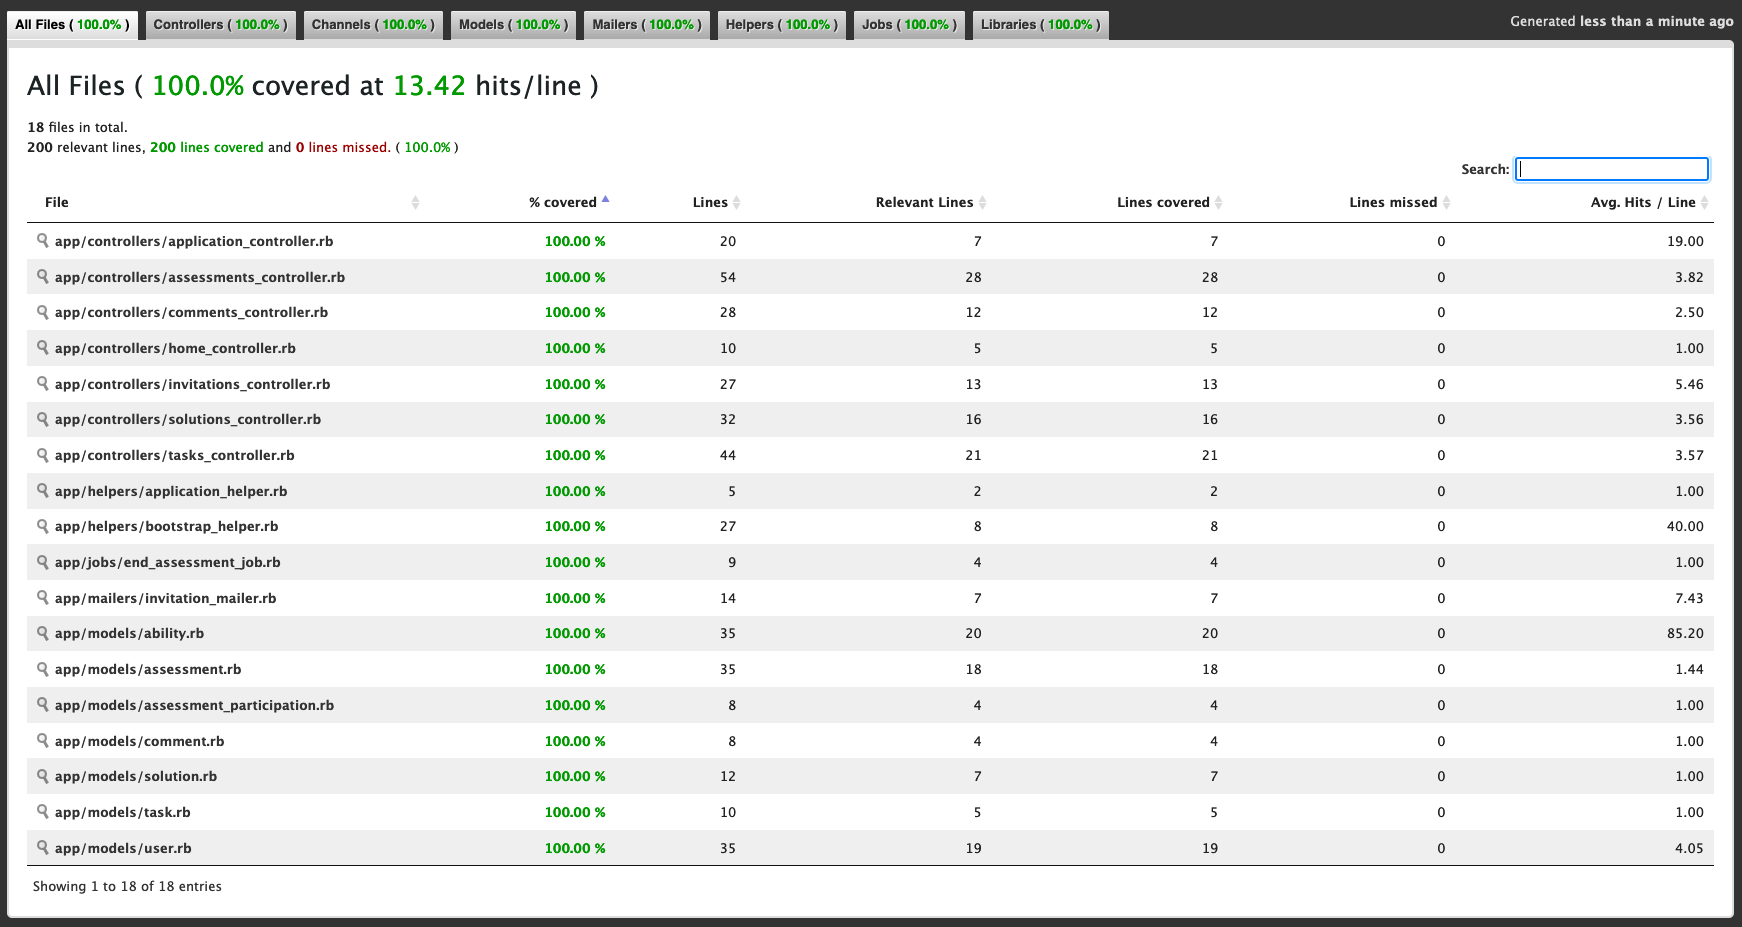
\includegraphics[width=\textwidth]{images/test-coverage.png}
  \caption{\label{fig:test-coverage}Erreichte \enquote{SimpleCov} Testabdeckung am 07.06.2022}
\end{figure}

Zusätzlich wurden planmässig alle Benutzer-Flows vollständig durch System-Tests gedeckt. Diese durchlaufen ebenfalls mit Erfolg und sind alle grün:

\begin{figure}[H]
  \centering
  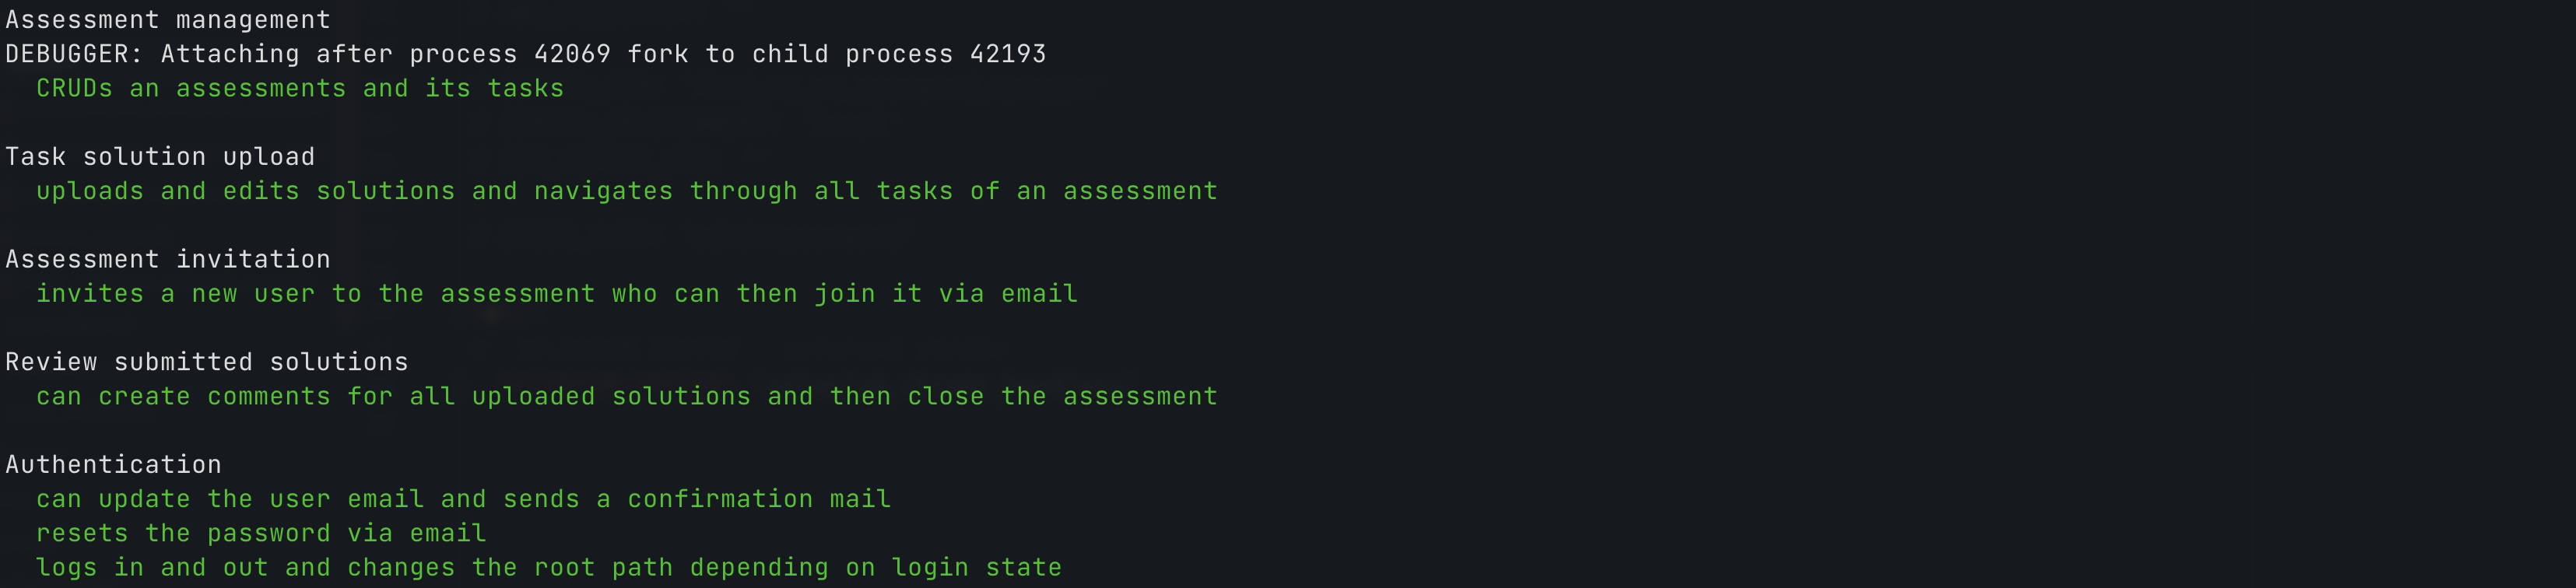
\includegraphics[width=\textwidth]{images/system-tests.png}
  \caption{\label{fig:system-tests}Durchlauf der Capybara System-Tets am 07.06.2022}
\end{figure}

\section{Linting-Checks}

Bei jedem CI-run werden nicht nur die oberhalb genannten automatisierten Tests ausgeführt, sondern der Code unterzieht sich auch diversen Linting- und Security-Checks.
Auch diese durchlaufen mit Erfolg und wurden an keiner Stelle im Code ignoriert. Damit entspricht der Ruby Code-Style in dieser PA vollständig den Rubocop-Guidelines.

\begin{figure}[H]
  \centering
  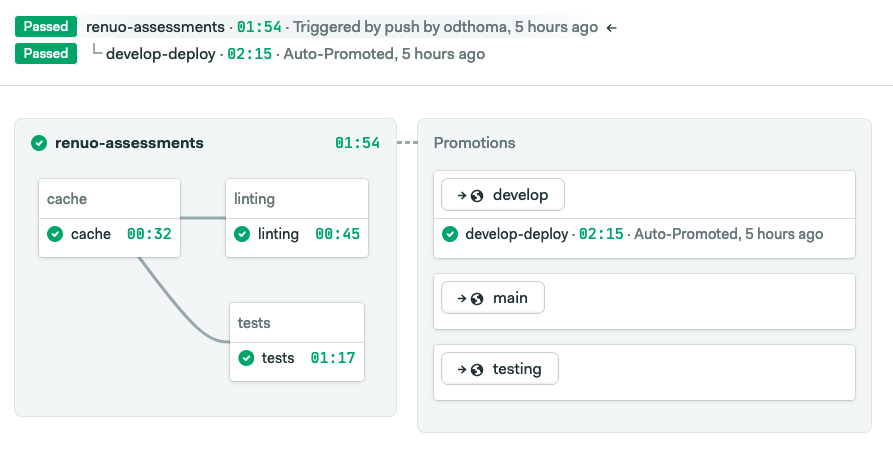
\includegraphics[width=\textwidth]{images/ci.png}
  \caption{\label{fig:semaphoreci}SemaphoreCI-Run vom letzten Git-Commit am 07.06.2022}
\end{figure}

\section{Manuelle Tests}

Auch die manuellen Tests konnten durch den Kandidaten, Oliver Thoma, mit Erfolg durchgeführt werden. Lediglich der Test \emph{ID 1} musste wiederholt werden, jedoch wurde beim zweiten Versuch
das erwartete Resultat erreicht. Ein korrektes Zusammenspiel aller Systeme auf der Produktions-Umgebung wurde somit sichergestellt.
Der Assessment-Assistant verhält sich dort nun genau so, wie auch schon auf der lokalen Umgebung des Kandidaten während der Entwicklungszeit.

\begin{table}[H]
  \begin{tabularx}{\linewidth}[H]{|c|l|l|X|}
    \hline
    \rowcolor{PrimaryColor!30} \textbf{Test-ID} & \textbf{Resultat} & \textbf{Datum und Uhrzeit} & \textbf{Bemerkungen}                                                                                          \\
    \hline
    1                                           & FAILED, SUCCESS   & 03.06.2022, 11:30 Uhr      & Dieser Test wurde aufgrund einer \gls{cors} Fehlkonfiguration auf der S3-development Instanz 2x durchgeführt. \\
    \hline
    2                                           & SUCCESS           & 06.06.2022, 13:30 Uhr      & Keine                                                                                                         \\
    \hline
    3                                           & SUCCESS           & 06.06.2022, 13:45 Uhr      & Keine                                                                                                         \\
    \hline
  \end{tabularx}
\end{table}

\chapter{Auswerten}

% see B6.6
% create a phantom toc entry for the index/glossary table
\clearpage\phantomsection\addcontentsline{toc}{part}{Glossar}

% generate glossary
\printnoidxglossary[title={Glossar}]

% create a phantom toc entry for the figures table
\clearpage\phantomsection\addcontentsline{toc}{part}{Abbildungsverzeichnis}

% generate figures table
\listoffigures

% create a phantom toc entry for the literature table
\clearpage\phantomsection\addcontentsline{toc}{part}{Literaturverzeichnis}

% generate bibliography
\printbibliography[title=Literaturverzeichnis]

% defines the beginning of the appendix
\appendix

% create a phantom toc entry for "Projekt"
\clearpage\phantomsection\addcontentsline{toc}{part}{Anhang}

% see B6.1b
\chapter{Quellcode}

\begin{figure}[H]
  \begin{codebox}[]
    \begin{minted}{javascript}
/**
 * @param {number} maxNumber
 * @return {number[]}
 */
 export default function sieveOfEratosthenes(maxNumber) {
  const isPrime = new Array(maxNumber + 1).fill(true);
  isPrime[0] = false;
  isPrime[1] = false;

  const primes = [];

  for (let number = 2; number <= maxNumber; number += 1) {
    if (isPrime[number] === true) {
      primes.push(number);

      /*
       * Optimisation.
       * Start marking multiples of `p` from `p * p`, and not from `2 * p`.
       * The reason why this works is because, at that point, smaller multiples
       * of `p` will have already been marked `false`.
       *
       * Warning: When working with really big numbers, the following line may cause overflow
       * In that case, it can be changed to:
       * let nextNumber = 2 * number;
       */
      let nextNumber = number * number;

      while (nextNumber <= maxNumber) {
        isPrime[nextNumber] = false;
        nextNumber += number;
      }
    }
  }

  return primes;
}
    \end{minted}
  \end{codebox}
  \caption[\enquote{Sieb des Eratosthenes implementiert mit JavaScript} visualisiert mit Minted]{Sieb des Eratosthenes implementiert mit JavaScript}
  \label{fig:sieve-of-eratosthenes}
\end{figure}

\end{document}
